%! TEX program = pdflatex
\documentclass[5p, twocolumn, times, sort&compress]{elsarticle}
\usepackage{url}  % to fix underscores in URLs in BibTex
\usepackage{amsmath}
\usepackage{amsthm}
\usepackage{amssymb}
\usepackage{amsfonts}
\usepackage{mathtools}
\usepackage[section]{placeins} % limit floats (figs, tables, etc.) to the same sections
\usepackage{tikz}  % visualizing computational graphs
\usepackage{relsize}  % setting font sizes relative to the current font size
\usepackage{makecell}  % create a multi-line cell
\usepackage{stfloats}  % for positioning of figure* on the same page
\usepackage{booktabs}  % table separation lines
\usepackage{threeparttable}  % three part table
\usepackage[group-separator={,}]{siunitx}  % unifying the styles of numbers, units, and quantities

% temporary; can be deleted
\usepackage{lipsum}  % generate random text as place holders

% helpful macros
\DeclareMathOperator*{\argmin}{arg\,min} % thin space, limits underneath in displays

% tikz setup
\input{tikzit.tikzstyles}

% figure-related
\graphicspath{{figs}}  % default figure search path
\DeclareGraphicsExtensions{.pdf,.png}  % priority of the formats of figures

% bibliography style
\bibliographystyle{elsarticle-num}

% journal name
\journal{Journal of Computational Science}

% main body
\begin{document}

    % front matter
    \begin{frontmatter}
        % title
        \title{%
            Predicting Fluid Dynamic Instabilities Using Physics-Informed Neural Networks%
        }

        % author list
        \author[1]{Pi-Yueh Chuang}
        \ead{pychuang@gwu.edu}
        \author[1]{Lorena A. Barba\corref{cor1}}
        \ead{labarba@gwu.edu}
        \cortext[cor1]{Corresponding author}
        \affiliation[1]{%
            organization={%
                Department of Mechanical and Aerospace Engineering, %
                The George Washington Unibersity%
            },%
            city={Washington},%
            state={DC 20052},%
            country={USA}%
        }

        % abstract
        \begin{abstract}
            \lipsum[1]%
        \end{abstract}

        % keywords
        \begin{keyword}
            computational fluid dynamics \sep
            physics-informed neural networks \sep
            dynamic mode analysis \sep
            koopman analysis \sep
            vortex shedding
        \end{keyword}
    \end{frontmatter}

    \section{Introduction}
    \lipsum[1-5] And \cite{chen_variants_2012, rowley_spectral_2009, rahaman_spectral_2019}.

    \section{Method}
    %! TEX root = main.tex

\lipsum[1]

\begin{figure*}[!t]
    \centering
    \normalsize
    \resizebox{\textwidth}{!}{\begin{tikzpicture}
	% network's frame
	\node [none] (network) at (0, 0) {
		Network
		$\left[\begin{smallmatrix} \vec{u} \\ p \end{smallmatrix}\right] =
		G(\vec{x}, t; \vec{\theta})$
	};

	% network's nodes: the input layer
	\node [below=1.5 of network.south west, input, anchor=north west] (nin1) {$x$};
	\node [below=0.5 of nin1, input] (nin2) {$y$};
	\node [below=0.5 of nin2, input] (nin3) {$t$};

	% network's nodes: the 1st hidden layer
	\node [right=0.3 of nin1, param] (nh12) {$h_2^1$};
	\node [above=0.5 of nh12, param] (nh11) {$h_1^1$};
	\node [below=0.5 of nh12, none]	(nh13) {$\vdots$};
	\node [below=0.5 of nh13, none]	(nh14) {$\vdots$};
	\node [below=0.5 of nh14, param] (nh15) {$h_{N_1}^1$};

	% network's nodes: the skipped layer
	\node [above right=0.3 of nh12, none]	(nskip1) {$\cdots$};
	\node [right=0.3 of nh13, none]	(nskip2) {$\cdots$};
	\node [above right=0.3 of nh15, none]	(nskip3) {$\cdots$};

	% network's nodes: the last hidden layer
	\node [right=0.6 of nh12, param] (nh22) {$h_2^\ell$};
	\node [above=0.5 of nh22, param] (nh21) {$h_1^\ell$};
	\node [below=0.5 of nh22, none]	(nh23) {$\vdots$};
	\node [below=0.5 of nh23, none]	(nh24) {$\vdots$};
	\node [below=0.5 of nh24, param] (nh25) {$h_{N_\ell}^\ell$};

	% network's nodes: the output layer
	\node [right=0.5 of nh22, input] (nout1) {$u$};
	\node [below=0.5 of nout1, input] (nout2) {$v$};
	\node [below=0.5 of nout2, input] (nout3) {$p$};

	% network's outer frame
	\node [draw=black!50, fit={(network) (nin2) (nh15) (nh25) (nout2)}] (nnframe){};

	% u derivative nodes
	\node [above right=1.6 and 0.8 of nout1.north east, anchor=south west, input] (dudt) {
		$\frac{\partial u}{\partial t}$};
	\node [right=0.1 of dudt.east, anchor=west, input] (dudx) {
		$\frac{\partial u}{\partial x}$};
	\node [right=0.1 of dudx.east, anchor=west, input] (dudy) {
		$\frac{\partial u}{\partial y}$};
	\node [right=0.1 of dudy.east, anchor=west, input] (d2udx2) {
		$\frac{\partial^2 u}{\partial x^2}$};
	\node [right=0.1 of d2udx2.east, anchor=west, input] (d2udy2) {
		$\frac{\partial^2 u}{\partial y^2}$};

	% u derivatives' outer frame
	\node [draw=black!50, fit={(dudt) (d2udy2)}] (dubox) {};

	% v derivative nodes
	\node [below right=1.2 and 0.8 of nout3.south east, anchor=north west, input] (dvdt) {
		$\frac{\partial v}{\partial t}$};
	\node [right=0.1 of dvdt.east, anchor=west, input] (dvdx) {
		$\frac{\partial v}{\partial x}$};
	\node [right=0.1 of dvdx.east, anchor=west, input] (dvdy) {
		$\frac{\partial v}{\partial y}$};
	\node [right=0.1 of dvdy.east, anchor=west, input] (d2vdx2) {
		$\frac{\partial^2 v}{\partial x^2}$};
	\node [right=0.1 of d2vdx2.east, anchor=west, input] (d2vdy2) {
		$\frac{\partial^2 v}{\partial y^2}$};

	% v derivatives' outer frame
	\node [draw=black!50, fit={(dvdt) (d2vdy2)}] (dvbox) {};

	% p derivative nodes
	\node [above=0.5 of dvdt.north west, anchor=south west, input] (dpdx) {
		$\frac{\partial p}{\partial x}$};
	\node [right=0.1 of dpdx.east, anchor=west, input] (dpdy) {
		$\frac{\partial p}{\partial y}$};

	% p derivatives' outer frame
	\node [draw=black!50, fit={(dpdx) (dpdy)}] (dpbox) {};

	% all derivatives' outer frame
	\node [draw=black!50, fit={(dubox) (dvbox)}] (dervbox) {};

	% loss 5: IC of v (rendered first bc it's at the center)
	\node [right=4.75 of nnframe.east, anchor=south west, input] (loss5) {$
		L_5 = v - v_0
		\text{\enspace if } t = 0
	$};

	% loss 4: IC of u
	\node [above=0.2 of loss5.north west, anchor=south west, input] (loss4) {$
		L_4 = u - u_0
		\text{\enspace if } t = 0
	$};

	% loss 3: momentum y
	\node [above=0.2 of loss4.north west, anchor=south west, input] (loss3) {$
		L_3 = 
			\frac{\partial v}{\partial t} +
			\vec{u} \cdot \nabla v +
			\frac{1}{\rho}\frac{\partial p}{\partial y} -
			\nu \nabla^2 v
		\text{\enspace if } \vec{x} \in {\Omega}
	$};

	% loss 2: momentum x
	\node [above=0.2 of loss3.north west, anchor=south west, input] (loss2) {$
		L_2 = 
			\frac{\partial u}{\partial t} +
			\vec{u} \cdot \nabla u +
			\frac{1}{\rho}\frac{\partial p}{\partial x} -
			\nu \nabla^2 u
		\text{\enspace if } \vec{x} \in {\Omega}
	$};

	% loss 1: continuity
	\node [above=0.2 of loss2.north west, anchor=south west, input] (loss1) {$
		L_1 = \nabla \cdot \vec{u} \text{\enspace if } \vec{x} \in {\Omega}
	$};

	% loss 6: IC of p
	\node [below=0.2 of loss5.south west, anchor=north west, input] (loss6) {$
		L_6 = p - p_0
		\text{\enspace if } t = 0
	$};

	% loss 7: dirichlet bc of u
	\node [below=0.2 of loss6.south west, anchor=north west, input] (loss7) {$
		L_7 = u - u_D \text{\enspace if } \vec{x}\in\Gamma_{\displaystyle u_D}
	$};

	% loss 8: dirichlet bc of v
	\node [below=0.2 of loss7.south west, anchor=north west, input] (loss8) {$
		L_8 = v - v_D \text{\enspace if } \vec{x}\in\Gamma_{\displaystyle v_D}
	$};

	% loss 9: neumann bc of u
	\node [below=0.2 of loss8.south west, anchor=north west, input] (loss9) {$
		L_9 = \frac{\partial u}{\partial \vec{n}} - u_N
		\text{\enspace if } \vec{x}\in\Gamma_{\displaystyle u_N}
	$};

	% loss 10: neumann bc of v
	\node [below=0.2 of loss9.south west, anchor=north west, input] (loss10) {$
		L_{10} = \frac{\partial v}{\partial \vec{n}} - v_N
		\text{\enspace if } \vec{x}\in\Gamma_{\displaystyle v_N}
	$};

	% losses' outer frame
	\node [draw=black!50, fit={(loss1) (loss2) (loss3) (loss10)}] (lossframe){};

	% arg min
	\node [right=0.5 of lossframe.east, anchor=west, input] (argmin) {$
		\argmin\limits_{\theta \in \Theta}
		\sum\limits_{\substack{\vec{x} \in \Omega \cup \Gamma \\ t \in T}}
		\sum\limits_{j=1}^{10} L_j^2
	$};
	\node [above=0.1 of argmin.north, anchor=south, none] (argmintxt) {Optimizing/training};

	% link network's inputs to the 1st hidden layer
	\draw [style=one arrow] (nin1) to (nh11);
	\draw [style=one arrow] (nin1) to (nh12);
	\draw [style=one arrow] (nin1) to (nh15);
	\draw [style=one arrow] (nin2) to (nh11);
	\draw [style=one arrow] (nin2) to (nh12);
	\draw [style=one arrow] (nin2) to (nh15);
	\draw [style=one arrow] (nin3) to (nh11);
	\draw [style=one arrow] (nin3) to (nh12);
	\draw [style=one arrow] (nin3) to (nh15);

	% link network's last hidden layer to the outputs
	\draw [style=one arrow] (nh21) to (nout1);
	\draw [style=one arrow] (nh21) to (nout2);
	\draw [style=one arrow] (nh21) to (nout3);
	\draw [style=one arrow] (nh22) to (nout1);
	\draw [style=one arrow] (nh22) to (nout2);
	\draw [style=one arrow] (nh22) to (nout3);
	\draw [style=one arrow] (nh25) to (nout1);
	\draw [style=one arrow] (nh25) to (nout2);
	\draw [style=one arrow] (nh25) to (nout3);

	% link network's outputs to derivatives
	\draw [style=one arrow] (nout1.east) to (dubox.west);
	\draw [style=one arrow] (nout2.east) to (dvbox.west);
	\draw [style=one arrow] (nout3.east) to (dpbox.west);

	% links to continuity loss
	\draw [style=one arrow] (dubox.east) to (loss1.west);
	\draw [style=one arrow] (dvbox.east) to (loss1.west);

	% links to x momemtum loss
	\draw [style=one arrow] (nout1.east) to (loss2.west);
	\draw [style=one arrow] (nout2.east) to (loss2.west);
	\draw [style=one arrow] (dubox.east) to (loss2.west);
	\draw [style=one arrow] (dvbox.east) to (loss2.west);
	\draw [style=one arrow] (dpbox.east) to (loss2.west);

	% links to y momemtum loss
	\draw [style=one arrow] (nout1.east) to (loss3.west);
	\draw [style=one arrow] (nout2.east) to (loss3.west);
	\draw [style=one arrow] (dubox.east) to (loss3.west);
	\draw [style=one arrow] (dvbox.east) to (loss3.west);
	\draw [style=one arrow] (dpbox.east) to (loss3.west);

	% links to u IC
	\draw[style=one arrow] (nout1.east) to (loss4.west);

	% links to v IC
	\draw[style=one arrow] (nout2.east) to (loss5.west);

	% links to p IC
	\draw[style=one arrow] (nout3.east) to (loss6.west);

	% links to u velocity Dirichlet BC
	\draw [style=one arrow] (nout1.east) to (loss7.west);

	% links to v velocity Dirichlet BC
	\draw [style=one arrow] (nout2.east) to (loss8.west);

	% links to u velocity Neumann BC
	\draw [style=one arrow] (dubox.east) to (loss9.west);

	% links to v velocity Neumann BC
	\draw [style=one arrow] (dvbox.east) to (loss10.west);

	% links from losses to argmin
	\draw [style=one arrow] (lossframe.east) to (argmin.west);

	% denoting automatic derivation
	\node [above right=0.8 and 0.3 of nnframe.north, anchor=west, none] (adtxt) {
		Automatic differentiation
	};
	\draw [-, draw=black!50] (nnframe.north) |- (adtxt.west);
	\draw [-{Latex[length=4]}, draw=black!50] (adtxt.east) -| (dervbox.north);

\end{tikzpicture}
% vim:ft=tex:\unskip}
    \caption[
        A graphical demonstration of the workflow in PINNs
    ]{
        A graphical demonstration of the workflow in PINNs
    }
    \label{fig:pinn-workflow}
\end{figure*}

\lipsum[3-10]

% vim:ft=tex:


    \section{Results}
    %! TEX root = main.tex

\lipsum[1]

\subsection{Verification: 2D Taylor-Green Vortex, $Re=\num{100}$}

\lipsum[1]

\begin{figure}[!hbt]
    \centering%
    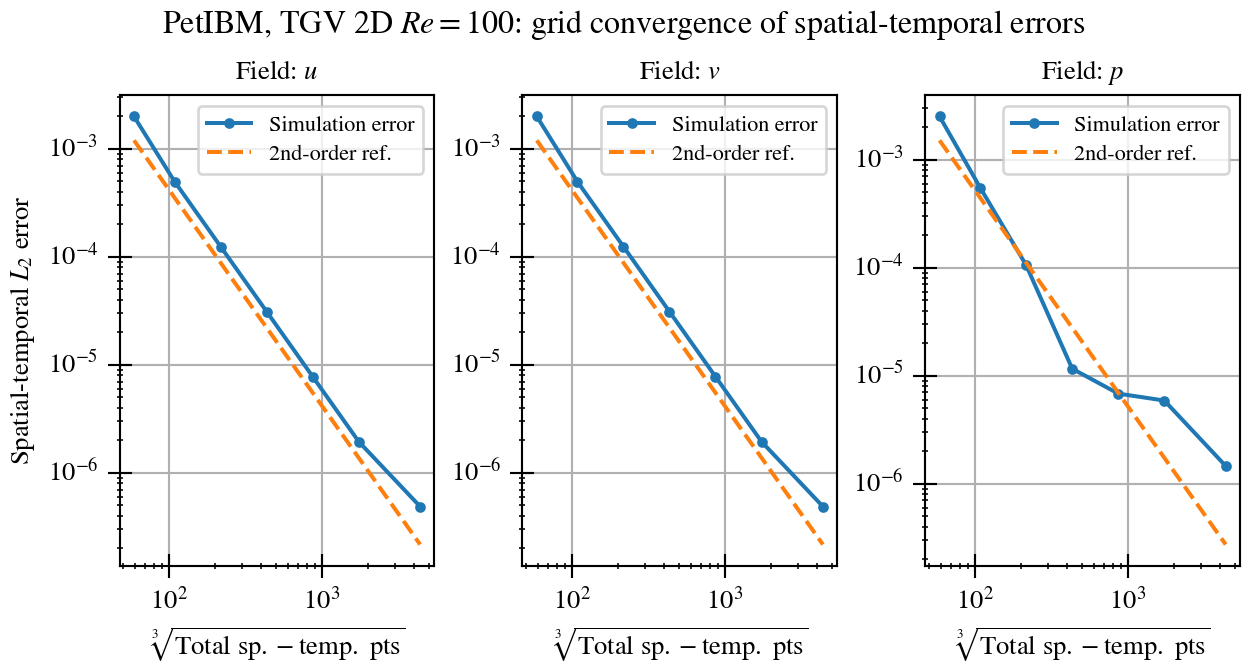
\includegraphics[width=\columnwidth]{tgv-2d-re100/petibm-tgv-2d-re100-convergence}%
    \caption{%
        Grid-convergence test of 2D TGV $Re=\num{100}$ w/ PetIBM
    }
    \label{fig:tgv-petibm-convergence}%
\end{figure}

\lipsum[1]

\begin{figure}[!hbt]
    \centering%
    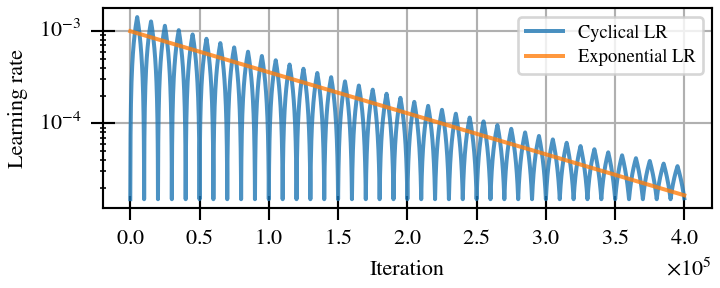
\includegraphics[width=\columnwidth]{tgv-2d-re100/learning-rate-hist}%
    \caption{%
        Learning-rate history of 2D TGV $Re=\num{100}$ w/ PINN
    }
    \label{fig:tgv-learning-rate-hist}%
\end{figure}

\lipsum[1]

\begin{figure}[!hbt]
    \centering%
    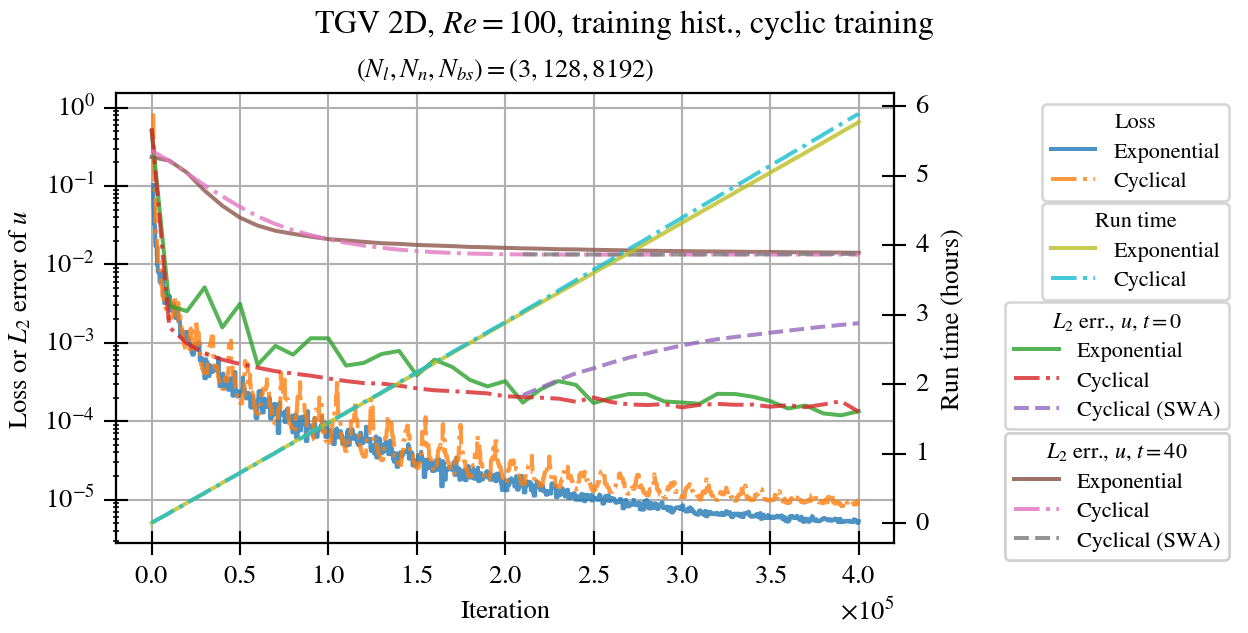
\includegraphics[width=\columnwidth]{tgv-2d-re100/pinn-nl3-nn128-npts8192-convergence}%
    \caption{%
        Training convergence history of 2D TGV $Re=\num{100}$ w/ PINN
    }
    \label{fig:tgv-pinn-loss}%
\end{figure}

\lipsum[1]

\begin{figure*}[!t]
    \centering%
    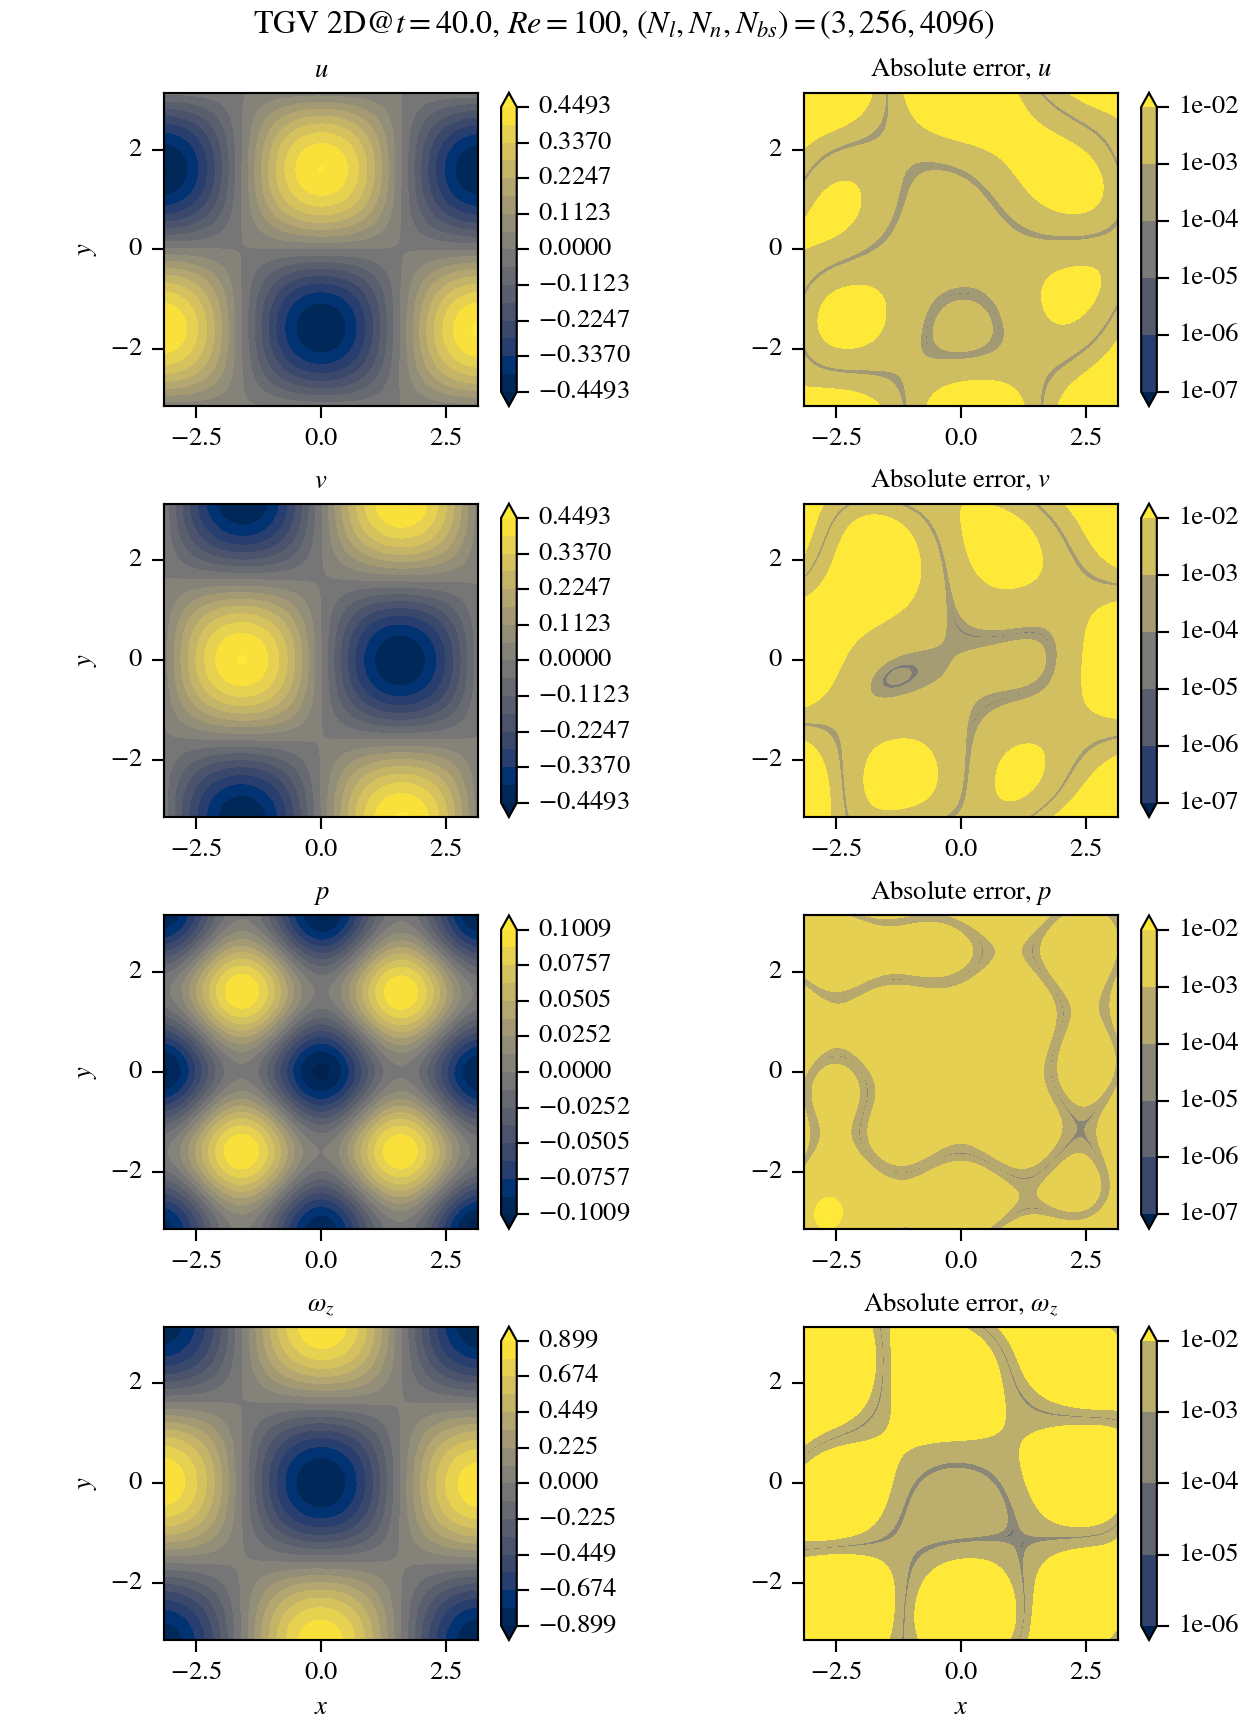
\includegraphics[width=0.8\linewidth]{tgv-2d-re100/pinn-nl3-nn256-npts4096-contours.png}%
    \caption{%
        Contours of 2D TGV $Re=\num{100}$ w/ PINN
    }
    \label{fig:tgv-pinn-contours}%
\end{figure*}

\lipsum[1]

\subsection{Verification and Validation: 2D Cylinder, $Re=\num{40}$}

\lipsum[1]

\begin{figure}[!hbt]
    \centering%
    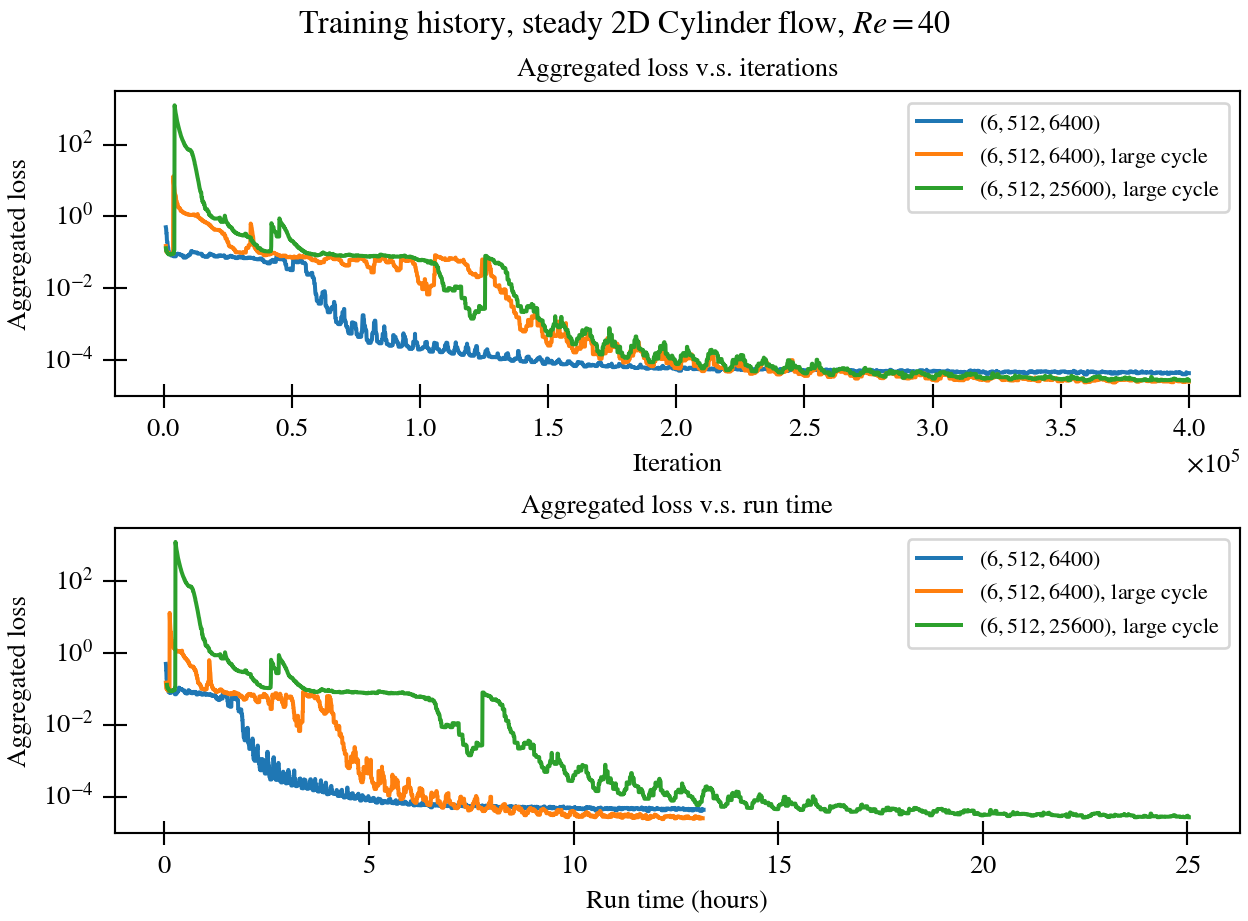
\includegraphics[width=0.95\columnwidth]{cylinder-2d-re40/loss-hist-steady.png}%
    \caption{%
        Training convergence history of 2D cylinder flow at $Re=\num{40}$ w/ steady PINN
    }
    \label{fig:cylinder-re40-steady-pinn-loss}%
\end{figure}

\lipsum[1]

\begin{figure}[!hbt]
    \centering%
    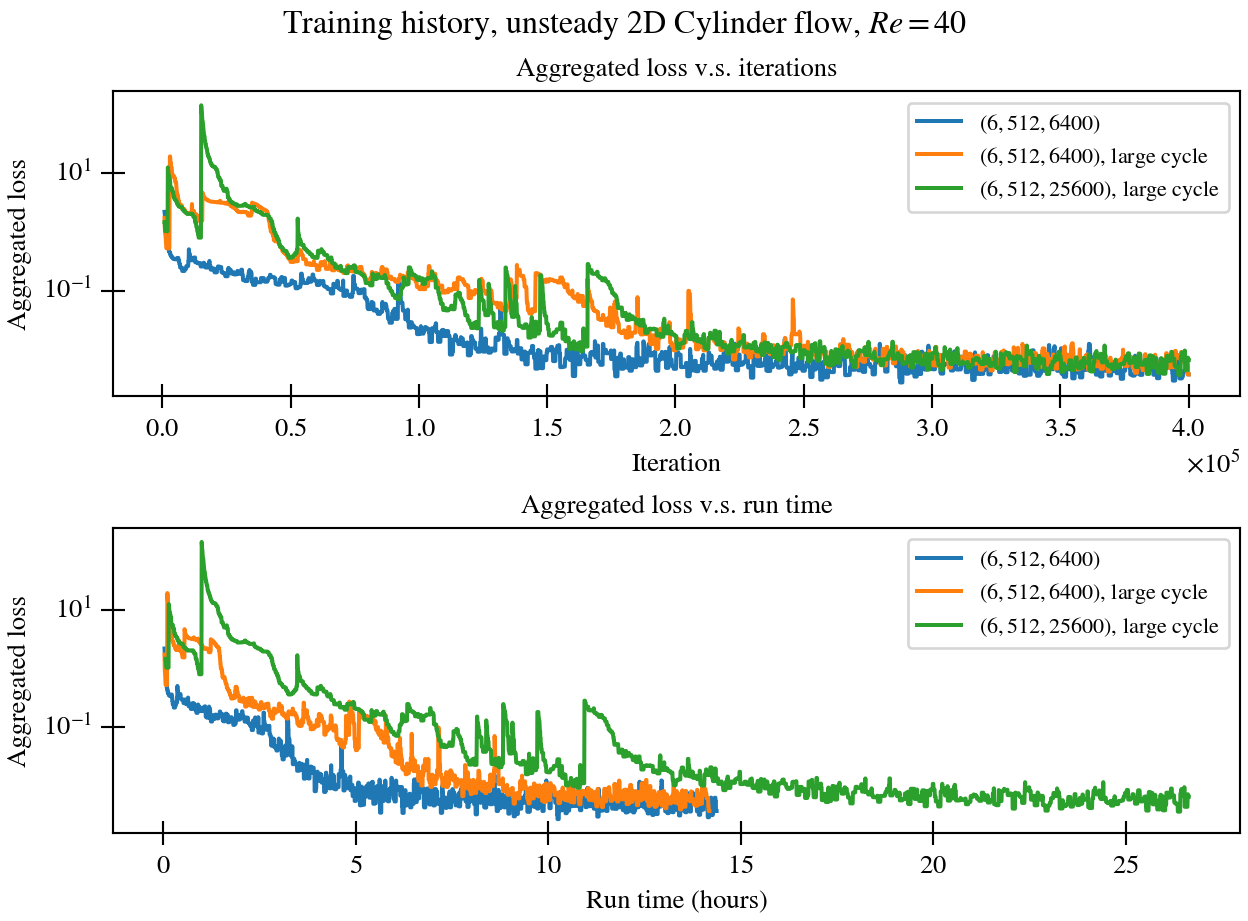
\includegraphics[width=0.95\columnwidth]{cylinder-2d-re40/loss-hist-unsteady.png}%
    \caption{%
        Training convergence history of 2D cylinder flow at $Re=\num{40}$ w/ unsteady PINN
    }
    \label{fig:cylinder-re40-unsteady-pinn-loss}%
\end{figure}

\lipsum[1]

\begin{table}[hbt!]
    \begin{threeparttable}[b]
        \begin{tabular}{lccc}
            \toprule
            & $C_D$ & $C_{D_p}$ & $C_{D_f}$ \\
            \midrule
            $(6, 512, 6400)$, steady & 1.62 & 1.07 & 0.55 \\
            $(6, 512, 6400)$, unsteady & 1.63 & 1.02 & 0.61 \\
            $(6, 512, 6400)$, large cycle, steady & 1.62 & 1.07 & 0.55 \\
            $(6, 512, 6400)$, large cycle, unsteady & 1.53 & 0.96 & 0.57 \\
            $(6, 512, 25600)$, large cycle, steady & 1.62 & 1.06 & 0.55 \\
            $(6, 512, 25600)$, large cycle, unsteady & 1.60 & 1.06 & 0.55 \\
            PetIBM & 1.63 & 1.02 & 0.61 \\
            Rosetti et al., 2012\cite{rosetti_urans_2012}\tnote{1} & \num{1.74+-0.09} & n/a & n/a \\
            Rosetti et al., 2012\cite{rosetti_urans_2012}\tnote{2} & 1.61 & n/a & n/a \\
            Sen et al., 2009\cite{sen_steady_2009}\tnote{2} & 1.51 & n/a & n/a \\
            Park et al., 1988\cite{park_numerical_1998}\tnote{2} & 1.51 & 0.99 & 0.53 \\
            Tritton, 1959\cite{tritton_experiments_1959}\tnote{1} & 1.48--1.65 & n/a & n/a \\
            Grove et al., 1964\cite{grove_experimental_1964}\tnote{1} & n/a & 0.94 & n/a \\
            \bottomrule
        \end{tabular}%
        \begin{tablenotes}
            \footnotesize
            \item [1] Experimental result
            \item [2] Simulation result
        \end{tablenotes}
        \caption{%
            Validation of drag coefficients.%
            $C_D$, $C_{D_p}$, and $C_{D_f}$ denote the coefficients of total drag, pressure drag, %
            and friction drag, respectively.%
        }%
        \label{table:cylinder-re40-cd-comparison}
    \end{threeparttable}
\end{table}%

\begin{figure}[!hbt]
    \centering%
    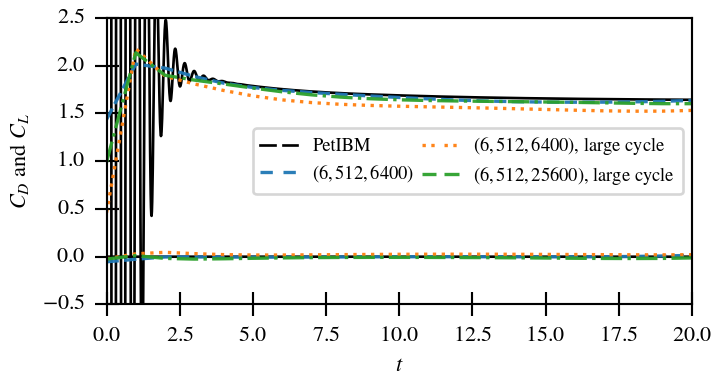
\includegraphics[width=0.95\columnwidth]{cylinder-2d-re40/drag-lift-coeffs}%
    \caption{%
        Drag and lift coefficients of 2D cylinder flow at $Re=\num{40}$ w/ PINNs
    }
    \label{fig:cylinder-re40-drag-lift}%
\end{figure}

\lipsum[1]

\begin{figure}[!hbt]
    \centering%
    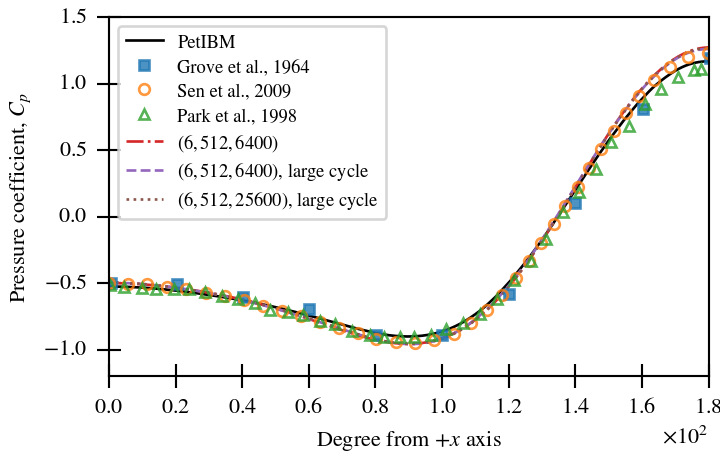
\includegraphics[width=0.95\columnwidth]{cylinder-2d-re40/surface-pressure-steady}%
    \caption{%
        Surface pressure distribution of 2D cylinder flow at $Re=\num{40}$ w/ steady PINN
    }
    \label{fig:cylinder-re40-steady-pinn-surfp}%
\end{figure}

\lipsum[1]

\begin{figure}[!hbt]
    \centering%
    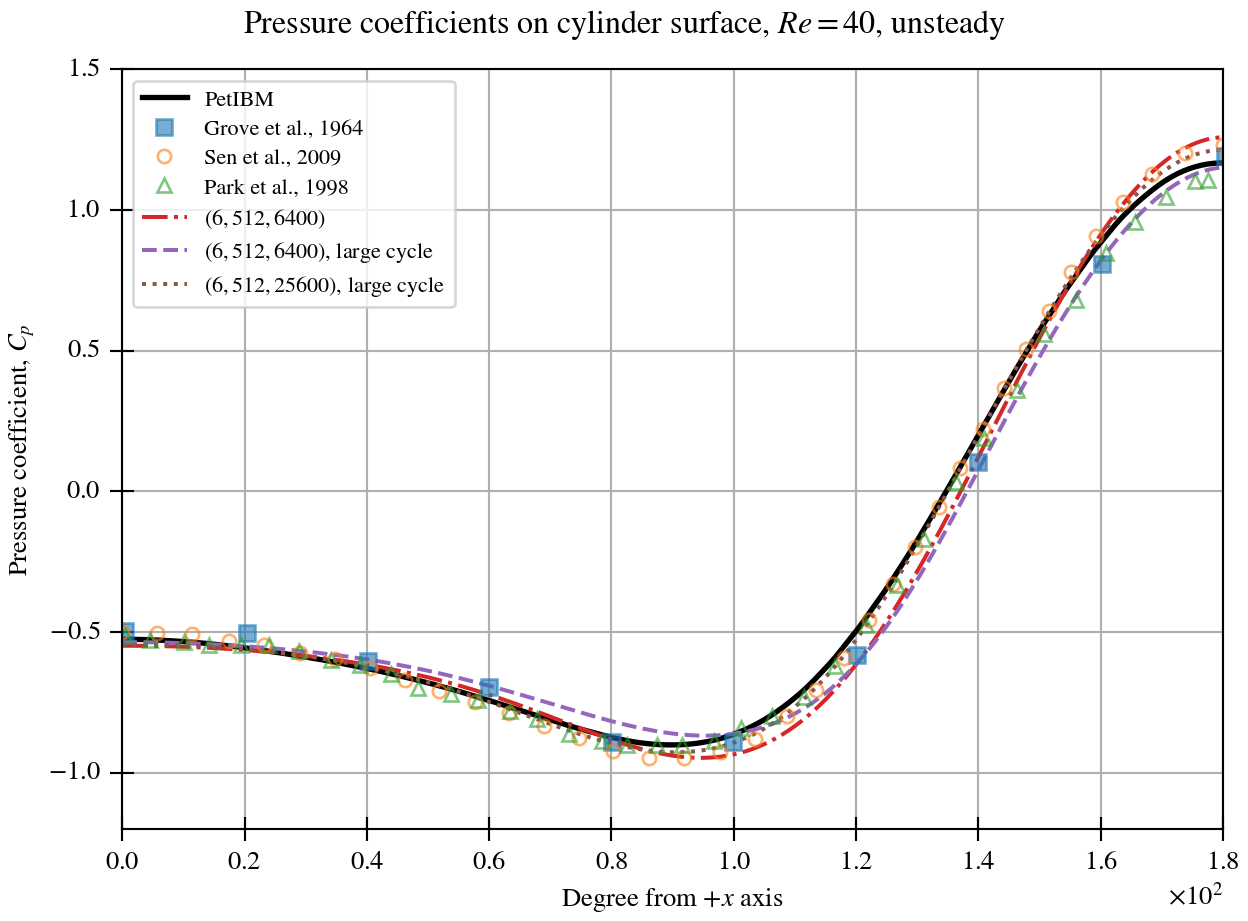
\includegraphics[width=0.95\columnwidth]{cylinder-2d-re40/surface-pressure-unsteady}%
    \caption{%
        Surface pressure distribution of 2D cylinder flow at $Re=\num{40}$ w/ unsteady PINN
    }
    \label{fig:cylinder-re40-unsteady-pinn-surfp}%
\end{figure}

\lipsum[1]

\begin{figure*}[!t]
    \centering%
    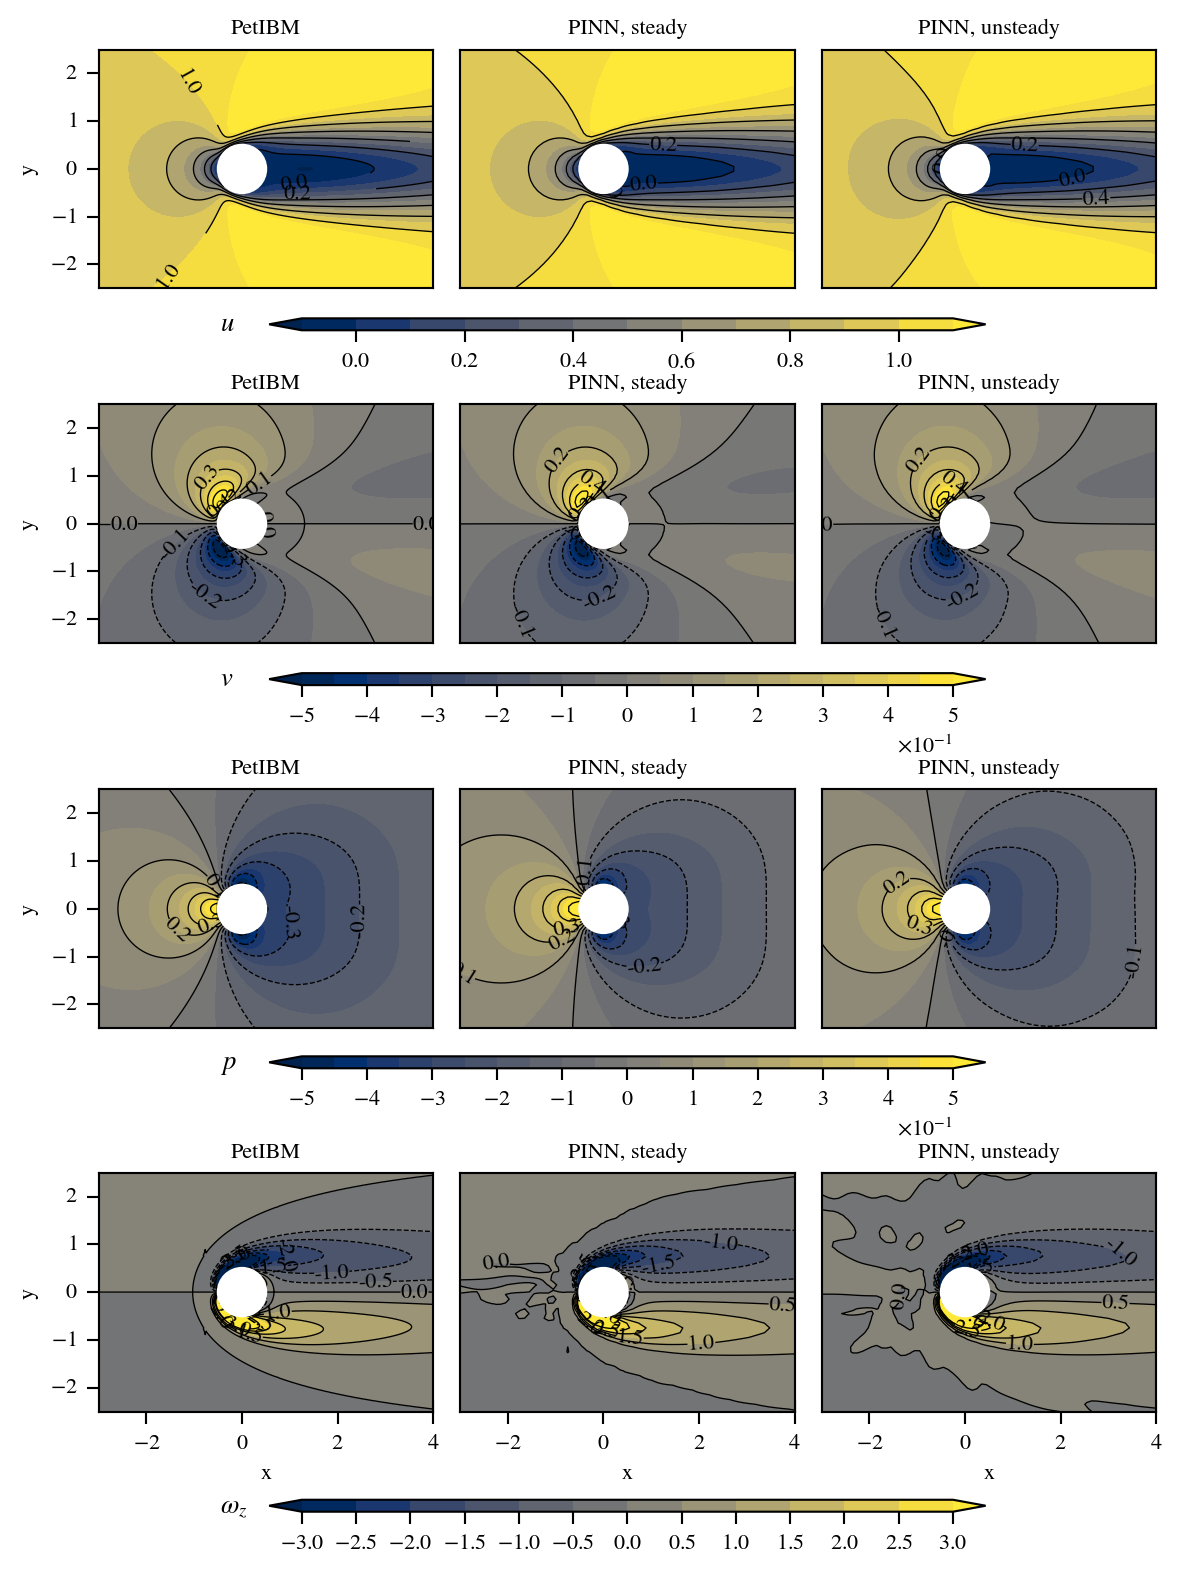
\includegraphics[width=0.85\linewidth]{cylinder-2d-re40/contour-comparison}%
    \caption{%
        Contour comparison of 2D cylinder flow at $Re=\num{40}$ w/ unsteady PINN
    }
    \label{fig:cylinder-re40-contours}%
\end{figure*}

\lipsum[1]

\subsection{2D Cylinder, $Re=\num{200}$}

\lipsum[1]

\begin{figure}[!hbt]
    \centering%
    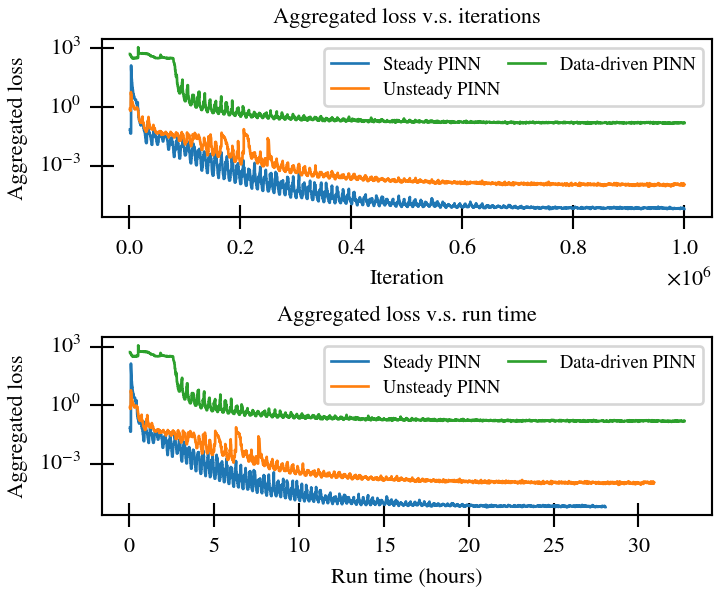
\includegraphics[width=0.95\columnwidth]{cylinder-2d-re200/loss-hist}%
    \caption{%
        Training convergence history of 2D cylinder flow at $Re=\num{200}$ w/ PINNs
    }
    \label{fig:cylinder-re200-pinn-loss}%
\end{figure}

\lipsum[1]

\begin{table}[hbt!]
    \begin{threeparttable}[b]
        \begin{tabular}{lcc}
            \toprule
            & $C_D$ \\
            \midrule
            PetIBM & 1.38   \\
            Steady PINN & 0.95 \\
            Unsteady PINN & 0.95 \\
            Deng et al., 2007\cite{deng_hydrodynamic_2007}\tnote{1} & 1.25 \\
            Rajani et al., 2009\cite{Rajani2009}\tnote{1} & 1.34 \\
            Gushchin \& Shchennikov, 1974\cite{gushchin_numerical_1974}\tnote{2} & 0.97 \\
            Fornberg, 1980\cite{fornberg_numerical_1980}\tnote{2} & 0.83 \\
            \bottomrule
        \end{tabular}%
        \begin{tablenotes}
            \footnotesize
            \item [1] Unsteady simulations.
            \item [2] Steady simulations.
        \end{tablenotes}
        \caption{%
            PINNs, 2D Cylinder, $Re=200$: validation of drag coefficients.%
            The data-driven case is excluded because it does not have an obvious periodic state nor a steady-state solution.%
        }%
        \label{table:cylinder-2d-re200-cd}
    \end{threeparttable}
\end{table}%

\begin{figure}[!hbt]
    \centering%
    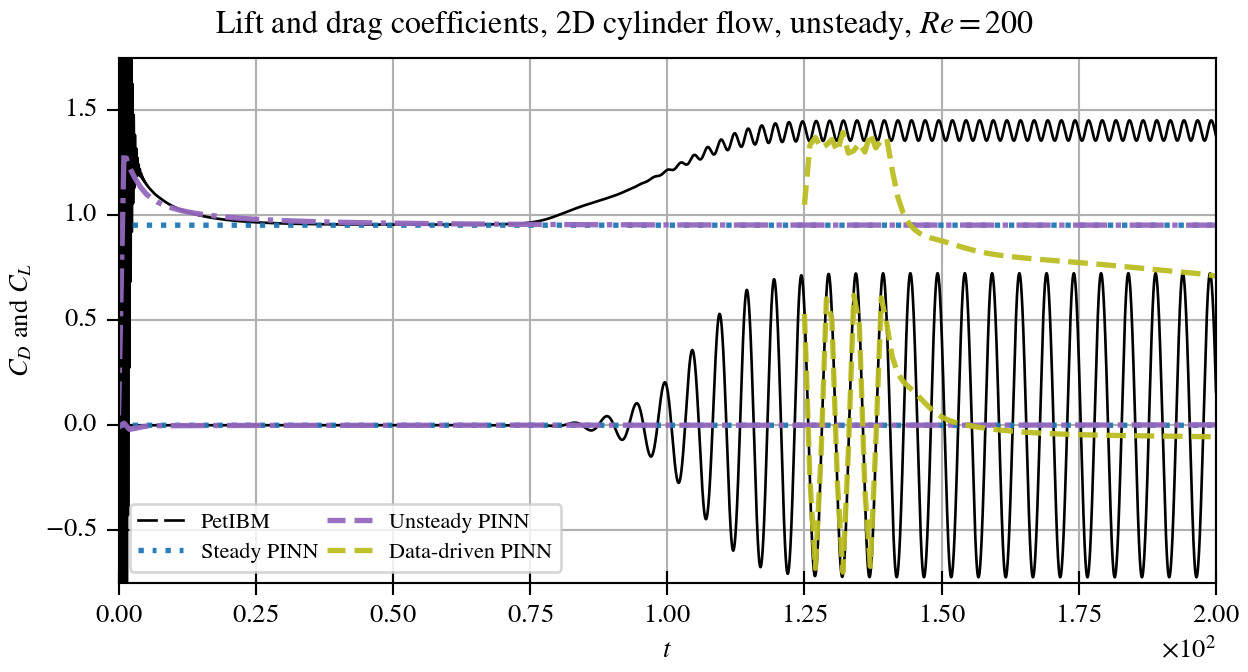
\includegraphics[width=0.95\columnwidth]{cylinder-2d-re200/drag-lift-coeffs}%
    \caption{%
        Drag and lift coefficients of 2D cylinder flow at $Re=\num{200}$ w/ PINNs
    }
    \label{fig:cylinder-re200-drag-lift}%
\end{figure}

\lipsum[1]

\begin{figure}[!hbt]
    \centering%
    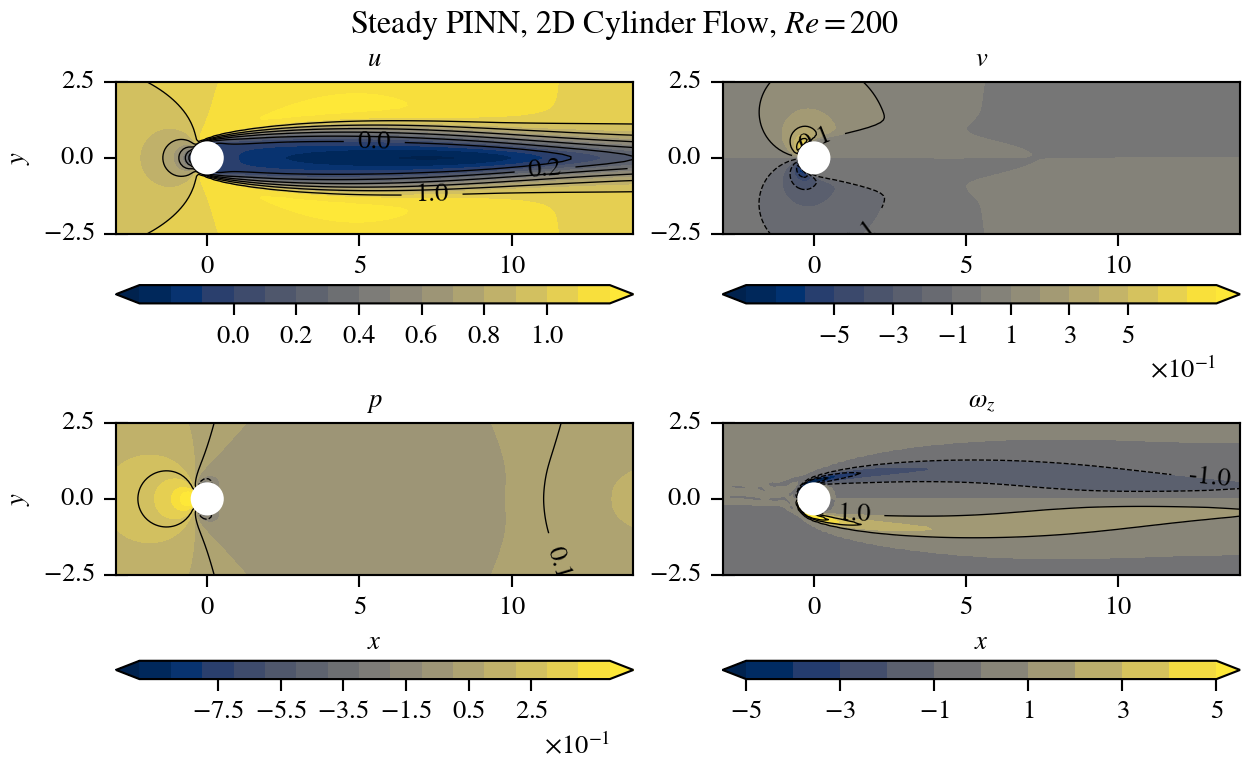
\includegraphics[width=0.95\columnwidth]{cylinder-2d-re200/contour-comparison-steady}%
    \caption{%
        Contours of 2D cylinder flow at $Re=\num{200}$ w/ steady PINN
    }
    \label{fig:cylinder-re200-steady-pinn-contours}%
\end{figure}

\begin{figure}[!hbt]
    \centering%
    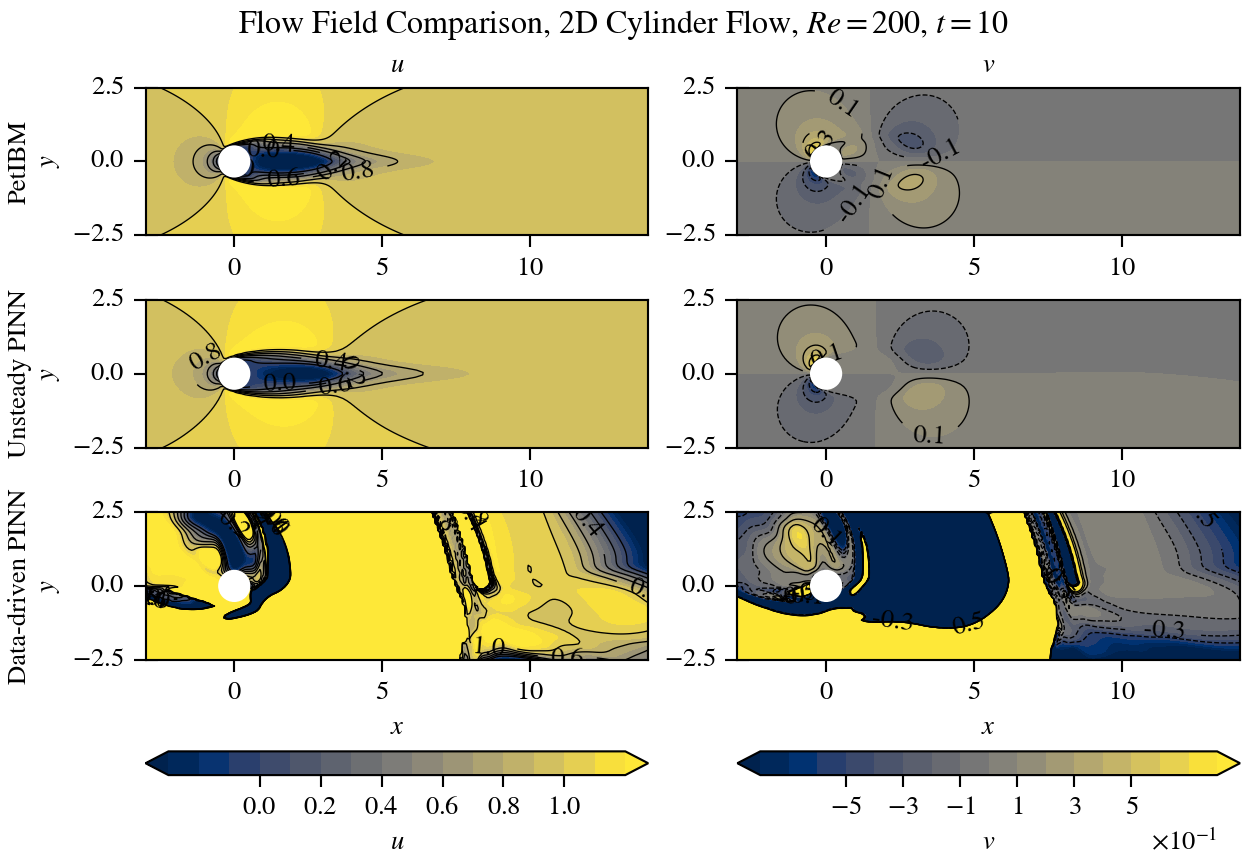
\includegraphics[width=0.95\columnwidth]{cylinder-2d-re200/contour-comparison-uv-t10}%
    \caption{%
        Contour comparison of 2D cylinder flow at $Re=\num{200}$ at $t=10$ w/ PINNs ($u$ and $v$ velocity)
    }
    \label{fig:cylinder-re200-pinn-contours-uv-t10}%
\end{figure}

\begin{figure}[!hbt]
    \centering%
    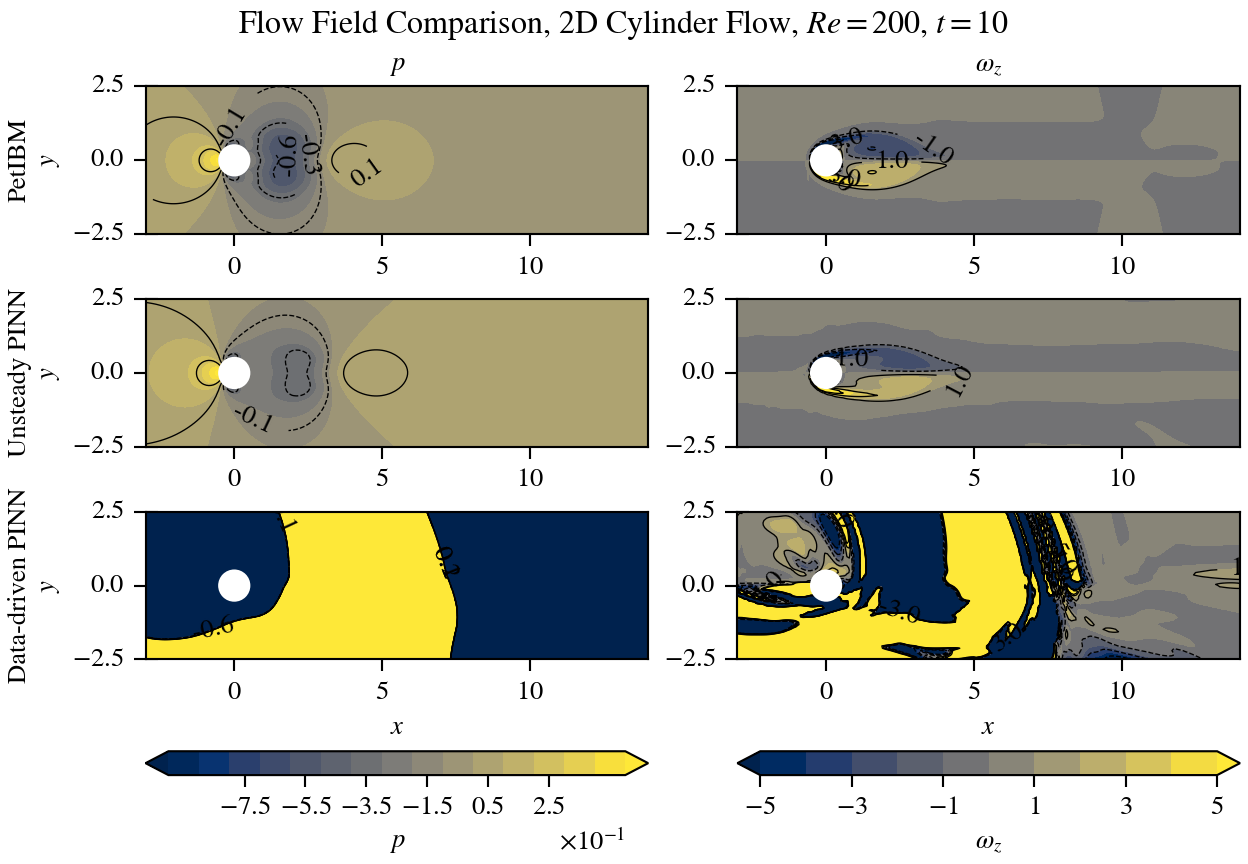
\includegraphics[width=0.95\columnwidth]{cylinder-2d-re200/contour-comparison-pwz-t10}%
    \caption{%
        Contour comparison of 2D cylinder flow at $Re=\num{200}$ at $t=10$ w/ PINNs (pressure and vorticity)
    }
    \label{fig:cylinder-re200-pinn-contours-pwz-t10}%
\end{figure}

\begin{figure}[!hbt]
    \centering%
    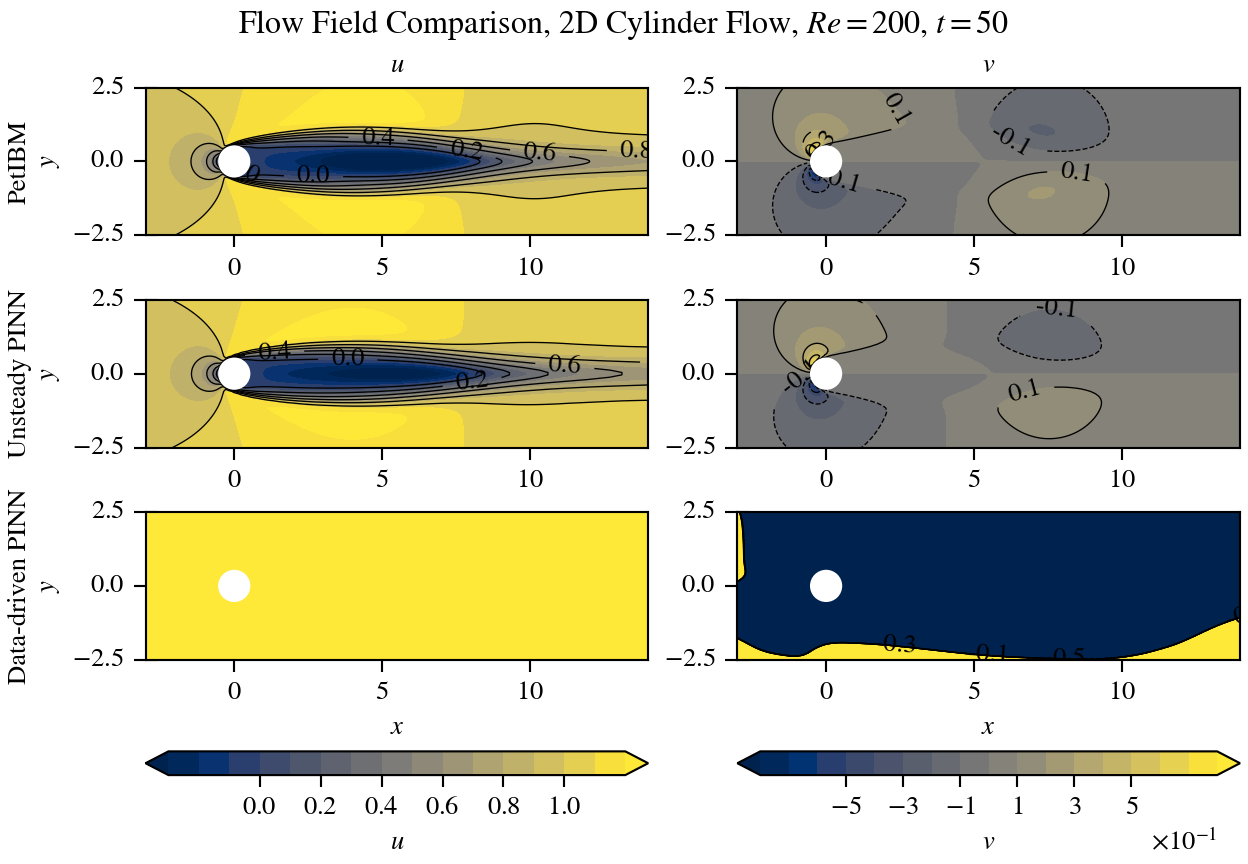
\includegraphics[width=0.95\columnwidth]{cylinder-2d-re200/contour-comparison-uv-t50}%
    \caption{%
        Contour comparison of 2D cylinder flow at $Re=\num{200}$ at $t=50$ w/ PINNs ($u$ and $v$ velocity)
    }
    \label{fig:cylinder-re200-pinn-contours-uv-t50}%
\end{figure}

\begin{figure}[!hbt]
    \centering%
    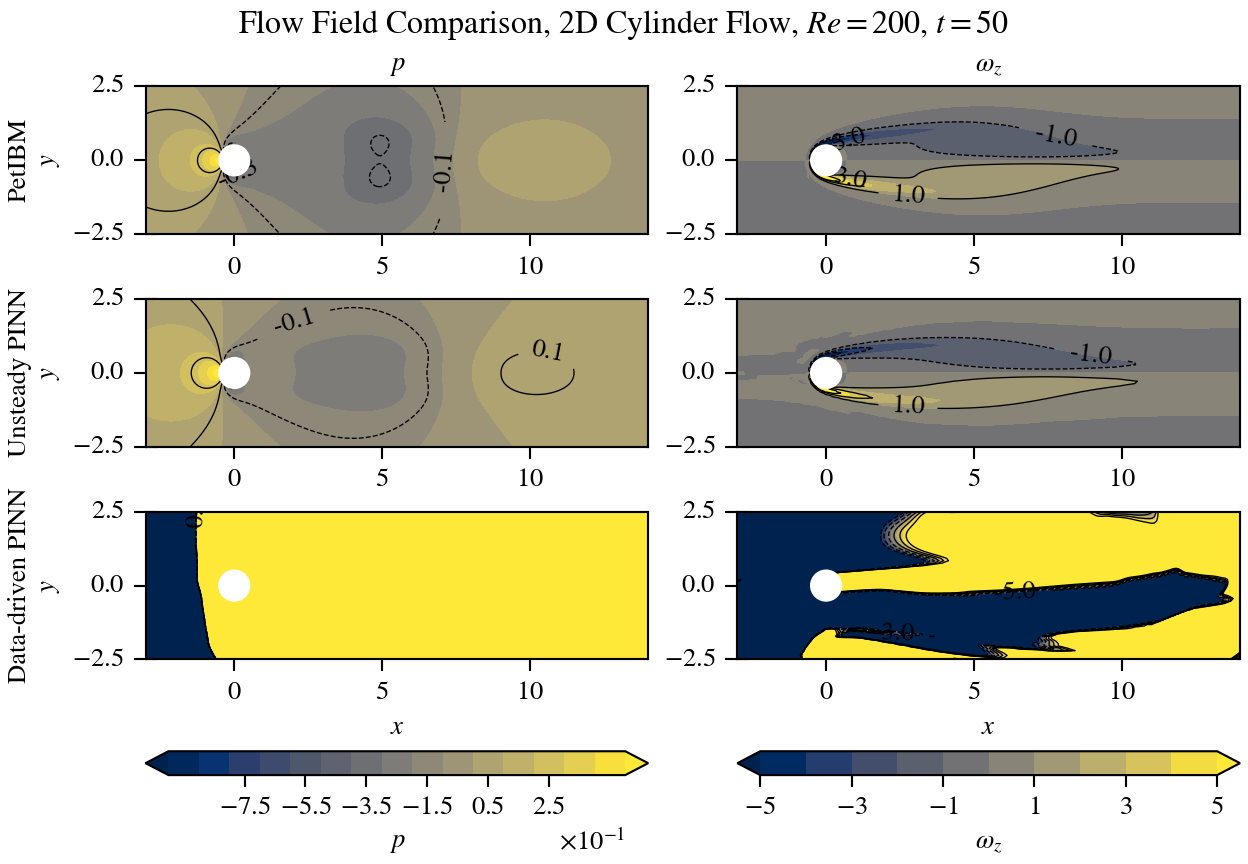
\includegraphics[width=0.95\columnwidth]{cylinder-2d-re200/contour-comparison-pwz-t50}%
    \caption{%
        Contour comparison of 2D cylinder flow at $Re=\num{200}$ at $t=50$ w/ PINNs (pressure and vorticity)
    }
    \label{fig:cylinder-re200-pinn-contours-pwz-t50}%
\end{figure}

\begin{figure}[!hbt]
    \centering%
    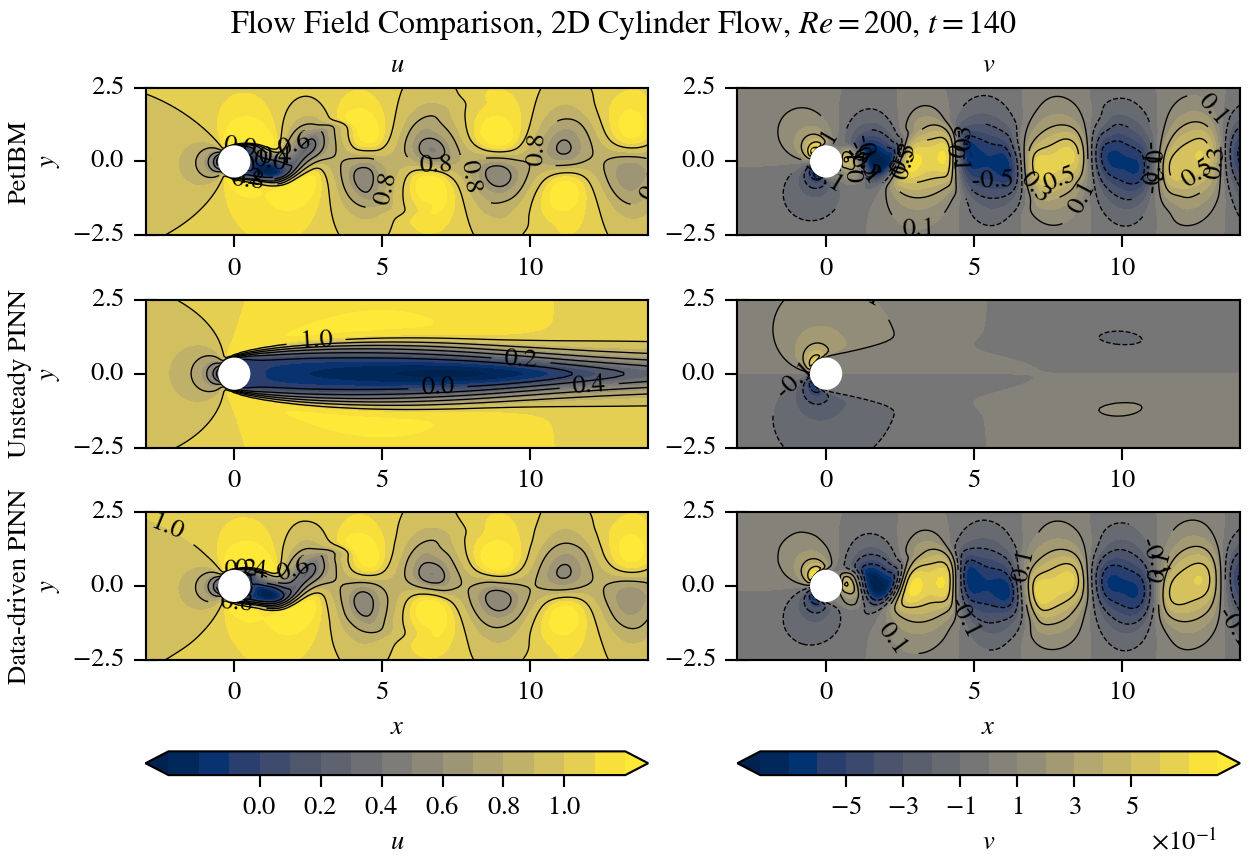
\includegraphics[width=0.95\columnwidth]{cylinder-2d-re200/contour-comparison-uv-t140}%
    \caption{%
        Contour comparison of 2D cylinder flow at $Re=\num{200}$ at $t=140$ w/ PINNs ($u$ and $v$ velocity)
    }
    \label{fig:cylinder-re200-pinn-contours-uv-t140}%
\end{figure}

\begin{figure}[!hbt]
    \centering%
    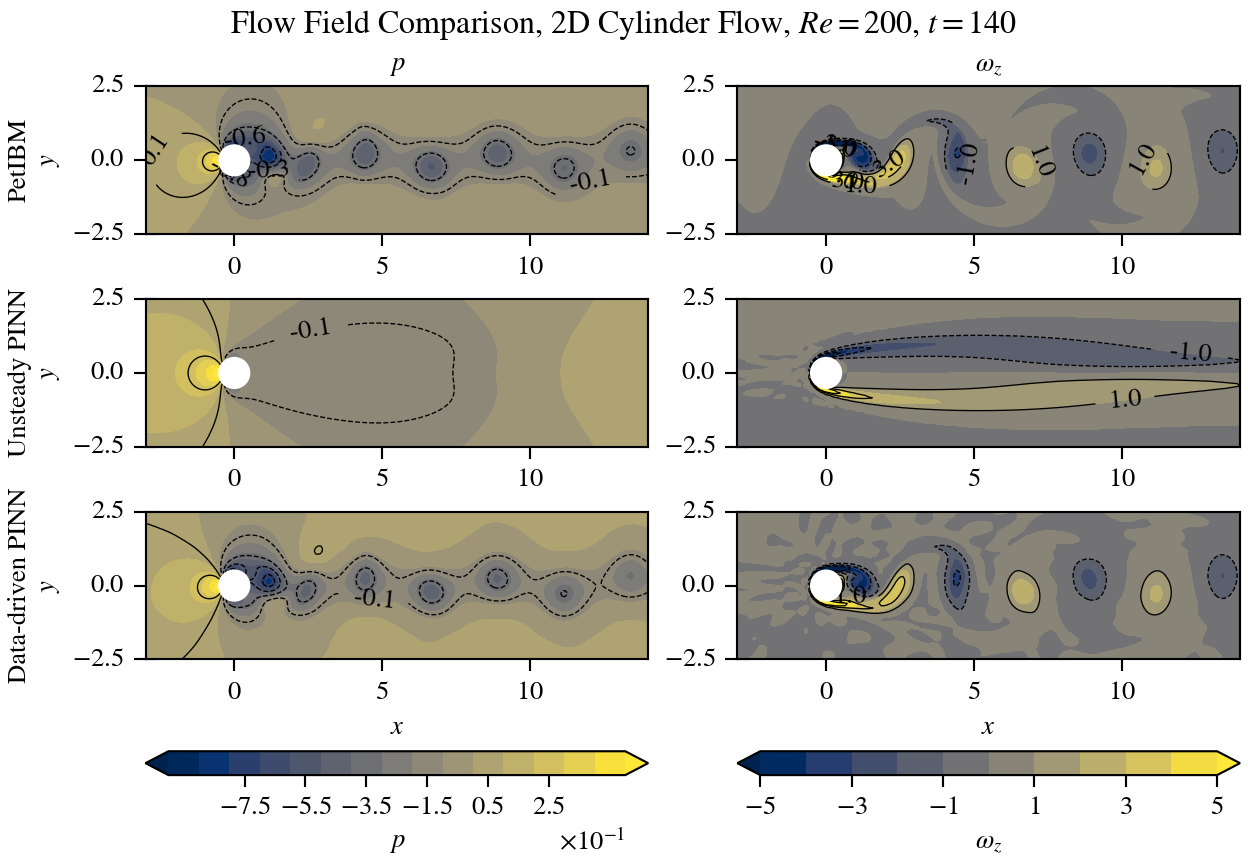
\includegraphics[width=0.95\columnwidth]{cylinder-2d-re200/contour-comparison-pwz-t140}%
    \caption{%
        Contour comparison of 2D cylinder flow at $Re=\num{200}$ at $t=140$ w/ PINNs (pressure and vorticity)
    }
    \label{fig:cylinder-re200-pinn-contours-pwz-t140}%
\end{figure}

\begin{figure}[!hbt]
    \centering%
    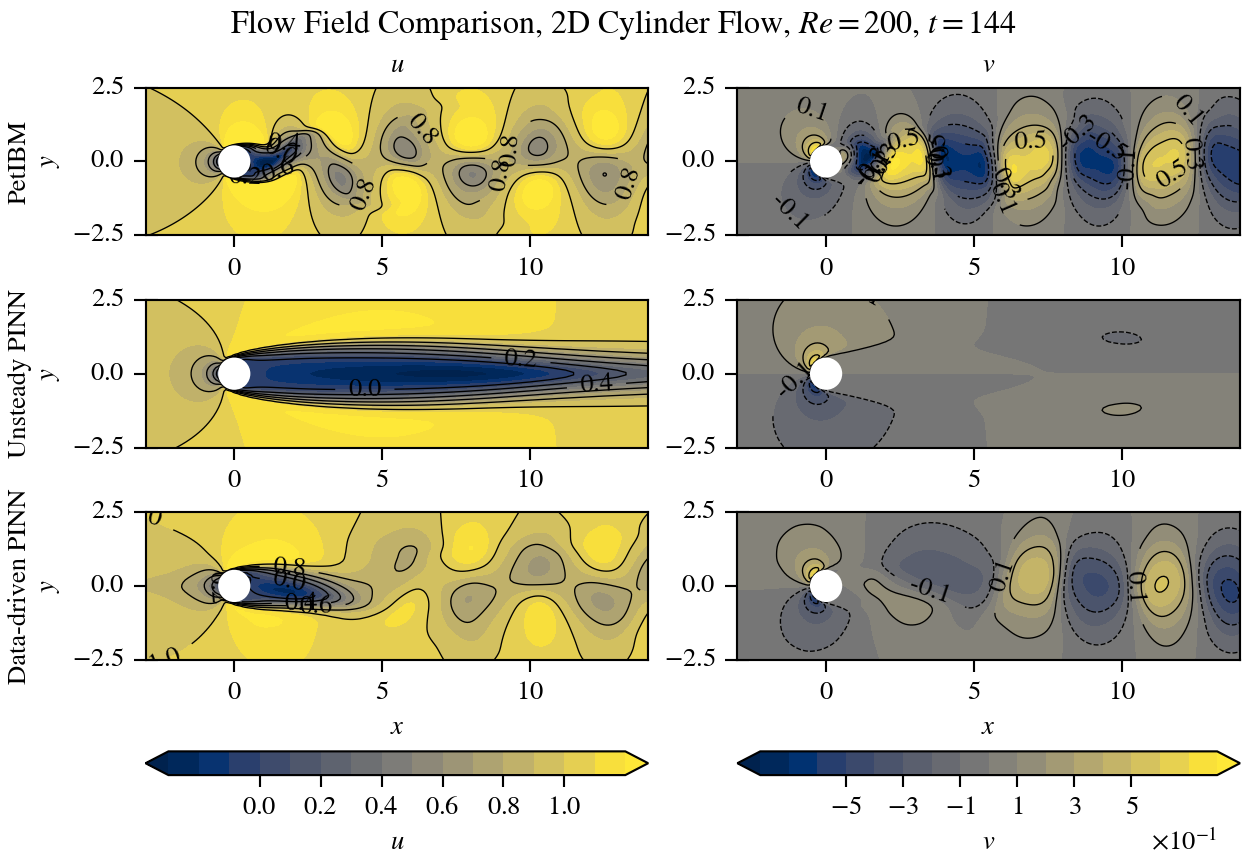
\includegraphics[width=0.95\columnwidth]{cylinder-2d-re200/contour-comparison-uv-t144}%
    \caption{%
        Contour comparison of 2D cylinder flow at $Re=\num{200}$ at $t=144$ w/ PINNs ($u$ and $v$ velocity)
    }
    \label{fig:cylinder-re200-pinn-contours-uv-t144}%
\end{figure}

\begin{figure}[!hbt]
    \centering%
    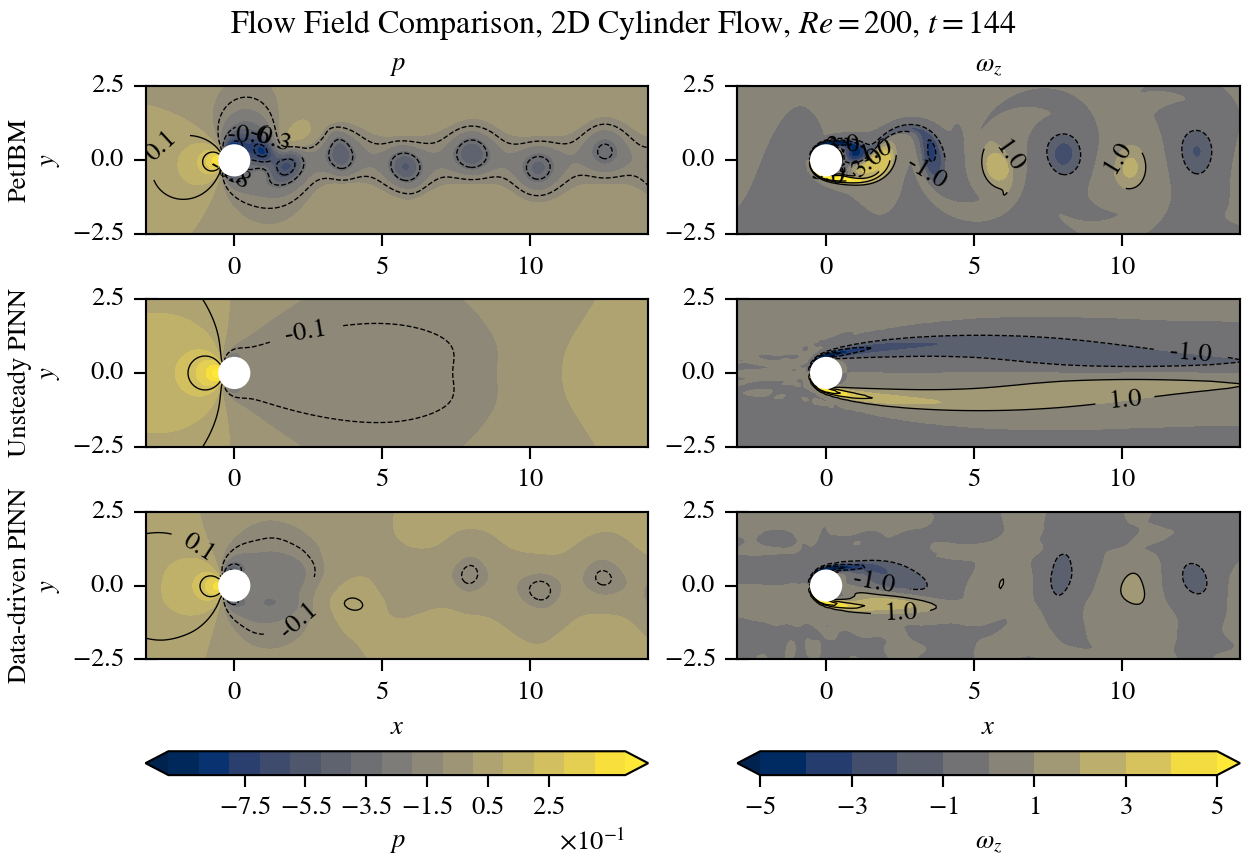
\includegraphics[width=0.95\columnwidth]{cylinder-2d-re200/contour-comparison-pwz-t144}%
    \caption{%
        Contour comparison of 2D cylinder flow at $Re=\num{200}$ at $t=144$ w/ PINNs (pressure and vorticity)
    }
    \label{fig:cylinder-re200-pinn-contours-pwz-t144}%
\end{figure}

\begin{figure}[!hbt]
    \centering%
    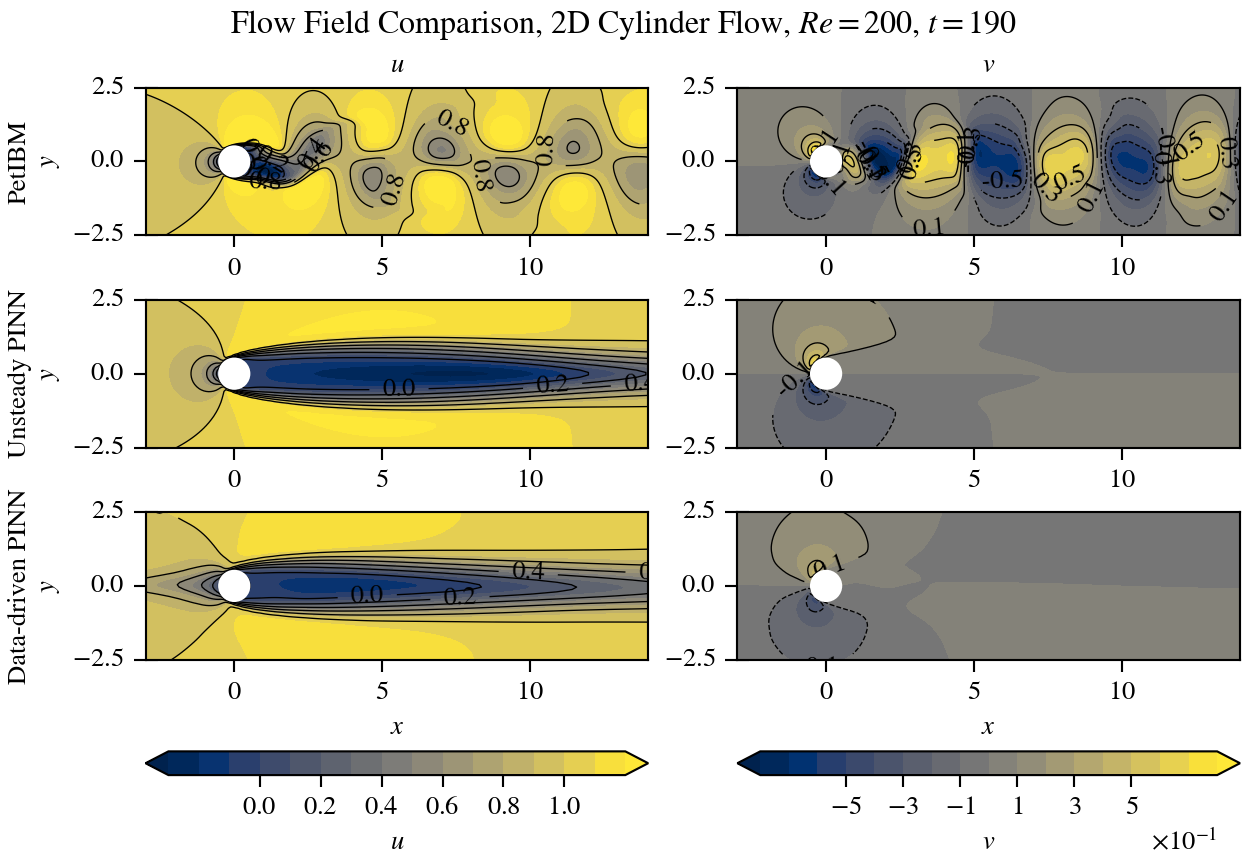
\includegraphics[width=0.95\columnwidth]{cylinder-2d-re200/contour-comparison-uv-t190}%
    \caption{%
        Contour comparison of 2D cylinder flow at $Re=\num{200}$ at $t=190$ w/ PINNs ($u$ and $v$ velocity)
    }
    \label{fig:cylinder-re200-pinn-contours-uv-t190}%
\end{figure}

\begin{figure}[!hbt]
    \centering%
    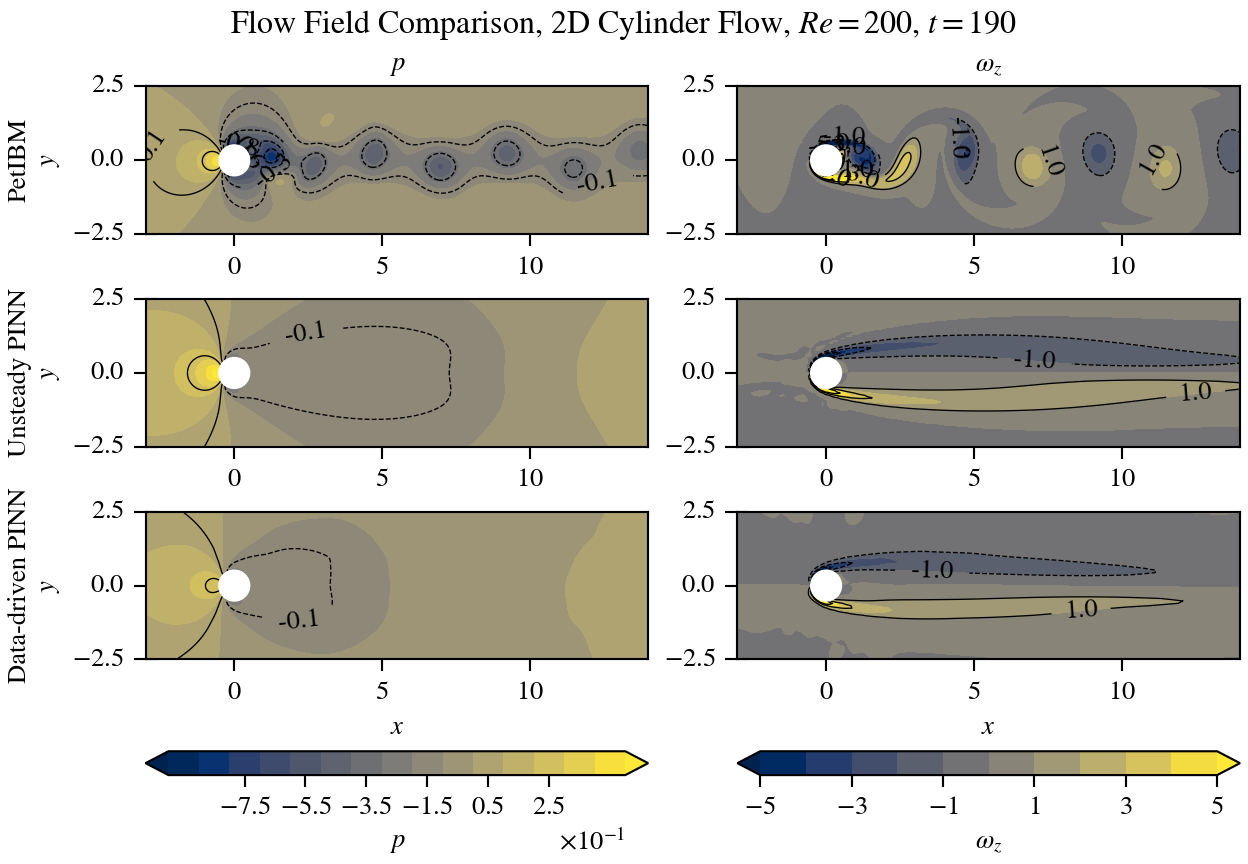
\includegraphics[width=0.95\columnwidth]{cylinder-2d-re200/contour-comparison-pwz-t190}%
    \caption{%
        Contour comparison of 2D cylinder flow at $Re=\num{200}$ at $t=190$ w/ PINNs (pressure and vorticity)
    }
    \label{fig:cylinder-re200-pinn-contours-pwz-t190}%
\end{figure}

\begin{figure}[!hbt]
    \centering%
    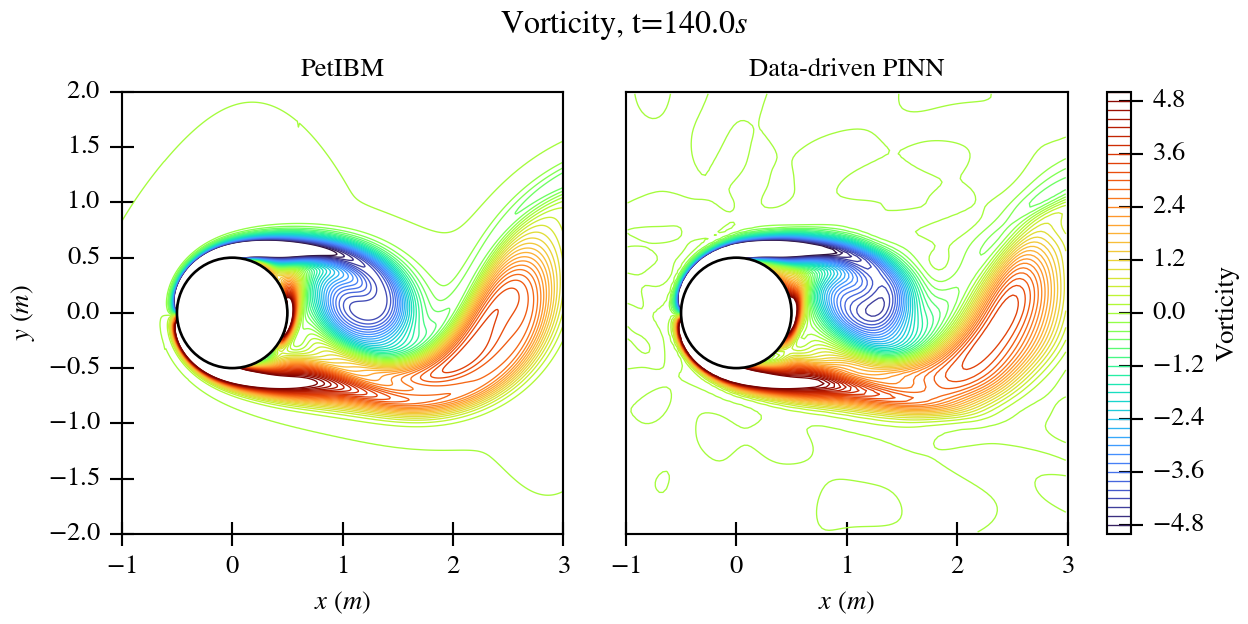
\includegraphics[width=0.95\columnwidth]{cylinder-2d-re200/vorticity_z_t140.0.png}%
    \caption{%
        Vorticity generation near the cylinder for 2D cylinder flow at $Re=\num{200}$ at $t=140$ w/ data-driven PINNs
    }
    \label{fig:cylinder-re200-pinn-vort-gen-t140.0}%
\end{figure}

\begin{figure}[!hbt]
    \centering%
    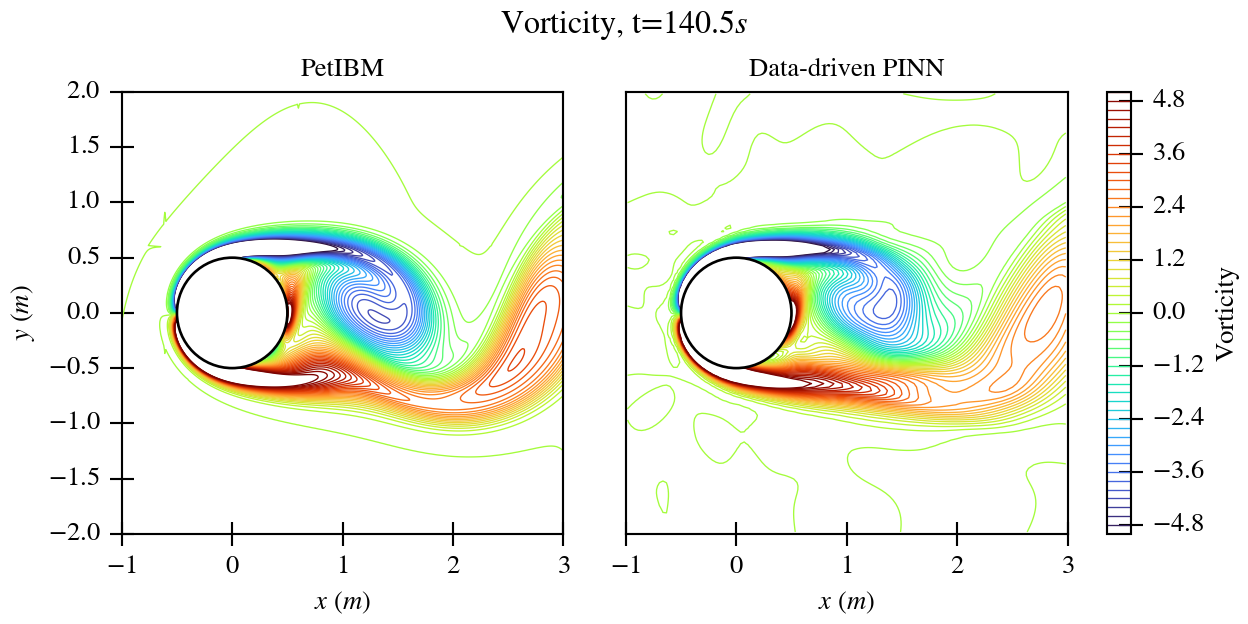
\includegraphics[width=0.95\columnwidth]{cylinder-2d-re200/vorticity_z_t140.5.png}%
    \caption{%
        Vorticity generation near the cylinder for 2D cylinder flow at $Re=\num{200}$ at $t=140.5$ w/ data-driven PINNs
    }
    \label{fig:cylinder-re200-pinn-vort-gen-t140.5}%
\end{figure}

\begin{figure}[!hbt]
    \centering%
    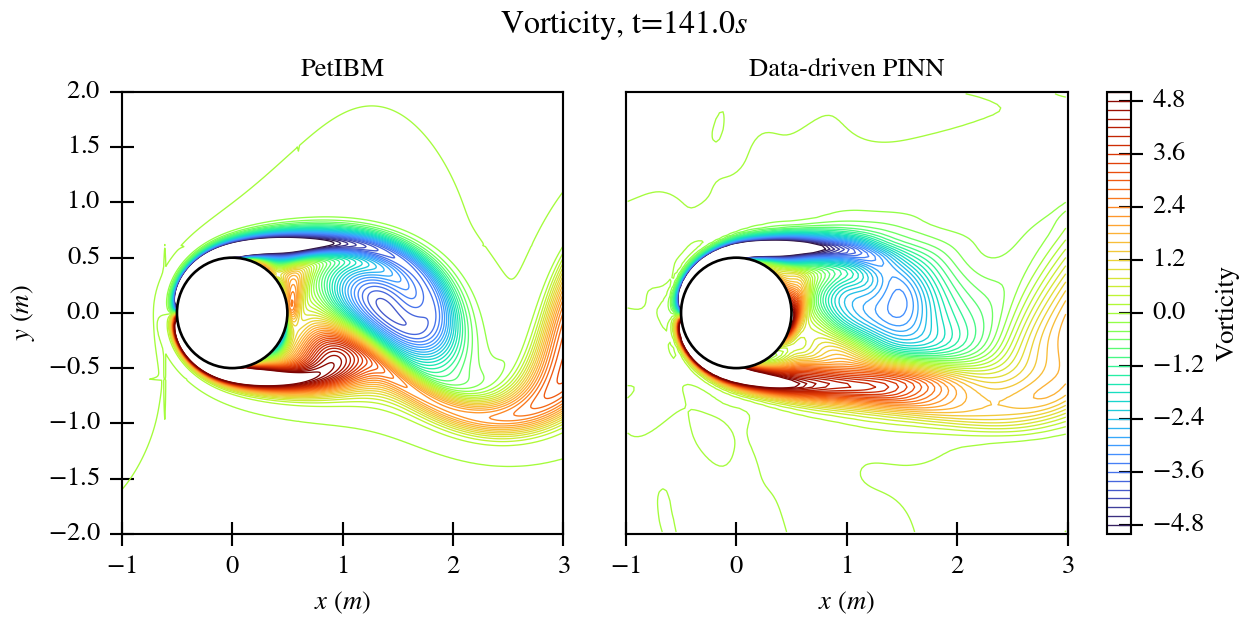
\includegraphics[width=0.95\columnwidth]{cylinder-2d-re200/vorticity_z_t141.0.png}%
    \caption{%
        Vorticity generation near the cylinder for 2D cylinder flow at $Re=\num{200}$ at $t=141$ w/ data-driven PINNs
    }
    \label{fig:cylinder-re200-pinn-vort-gen-t141.0}%
\end{figure}

\begin{figure}[!hbt]
    \centering%
    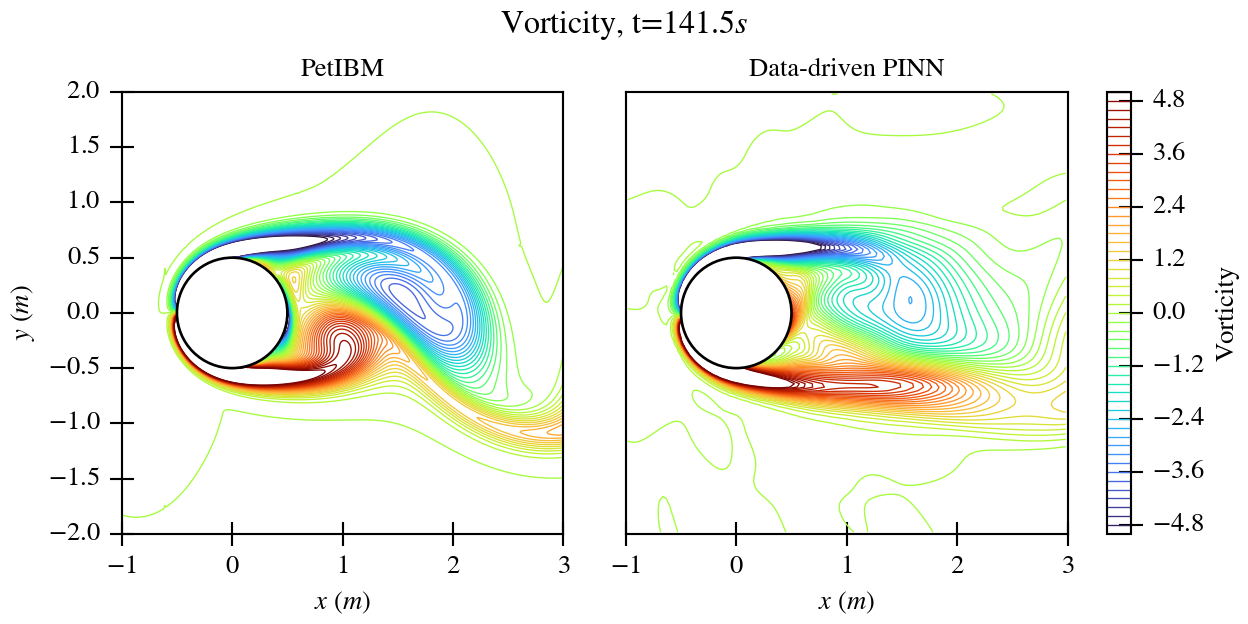
\includegraphics[width=0.95\columnwidth]{cylinder-2d-re200/vorticity_z_t141.5.png}%
    \caption{%
        Vorticity generation near the cylinder for 2D cylinder flow at $Re=\num{200}$ at $t=141.5$ w/ data-driven PINNs
    }
    \label{fig:cylinder-re200-pinn-vort-gen-t141.5}%
\end{figure}

\begin{figure}[!hbt]
    \centering%
    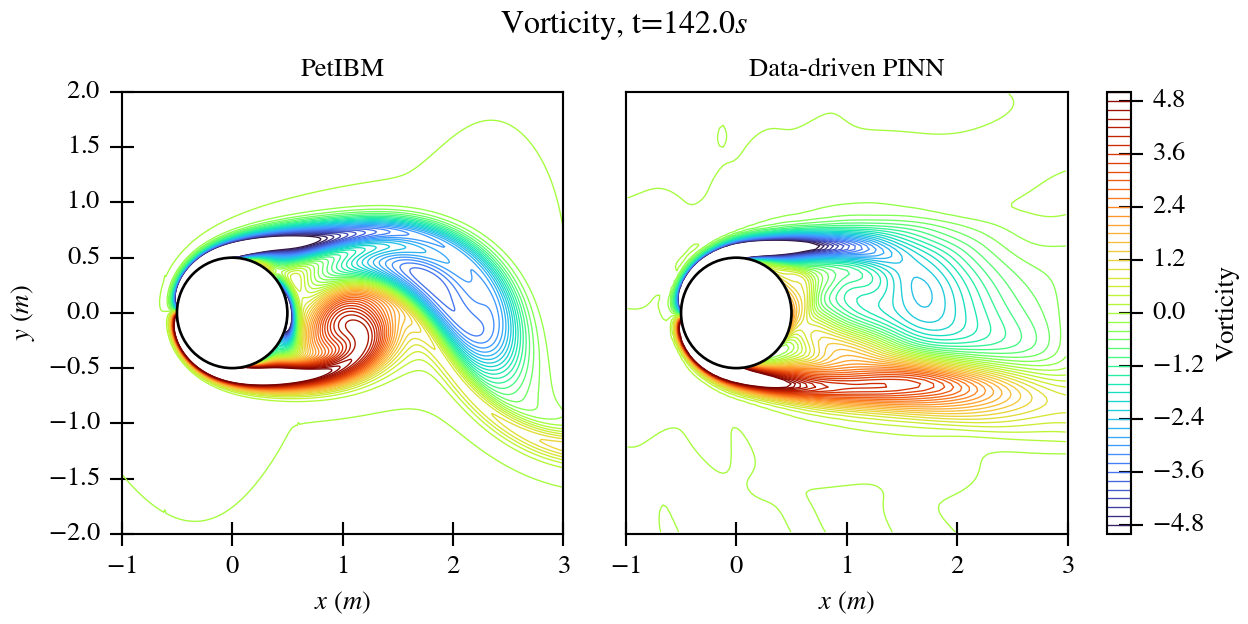
\includegraphics[width=0.95\columnwidth]{cylinder-2d-re200/vorticity_z_t142.0.png}%
    \caption{%
        Vorticity generation near the cylinder for 2D cylinder flow at $Re=\num{200}$ at $t=142$ w/ data-driven PINNs
    }
    \label{fig:cylinder-re200-pinn-vort-gen-t142.0}%
\end{figure}

\begin{figure}[!hbt]
    \centering%
    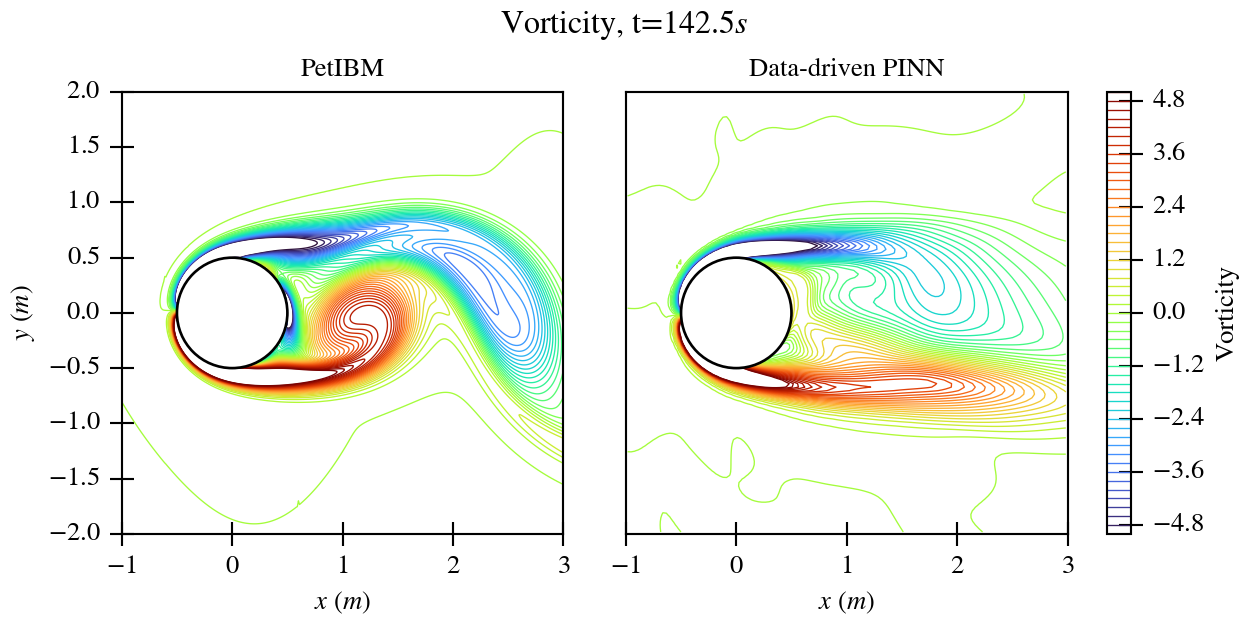
\includegraphics[width=0.95\columnwidth]{cylinder-2d-re200/vorticity_z_t142.5.png}%
    \caption{%
        Vorticity generation near the cylinder for 2D cylinder flow at $Re=\num{200}$ at $t=142.5$ w/ data-driven PINNs
    }
    \label{fig:cylinder-re200-pinn-vort-gen-t142.5}%
\end{figure}

\begin{figure}[!hbt]
    \centering%
    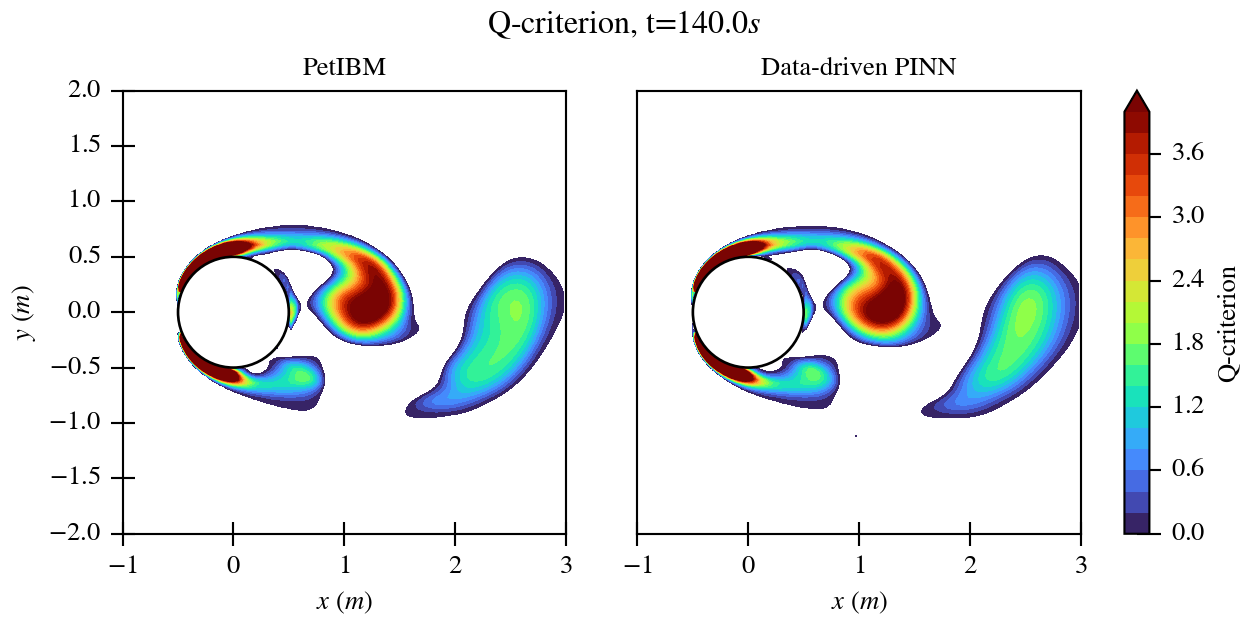
\includegraphics[width=0.95\columnwidth]{cylinder-2d-re200/qcriterion_t140.0.png}%
    \caption{%
        Q-criterion near the cylinder for 2D cylinder flow at $Re=\num{200}$ at $t=140$ w/ data-driven PINNs
    }
    \label{fig:cylinder-re200-pinn-qcrit-t140.0}%
\end{figure}

\begin{figure}[!hbt]
    \centering%
    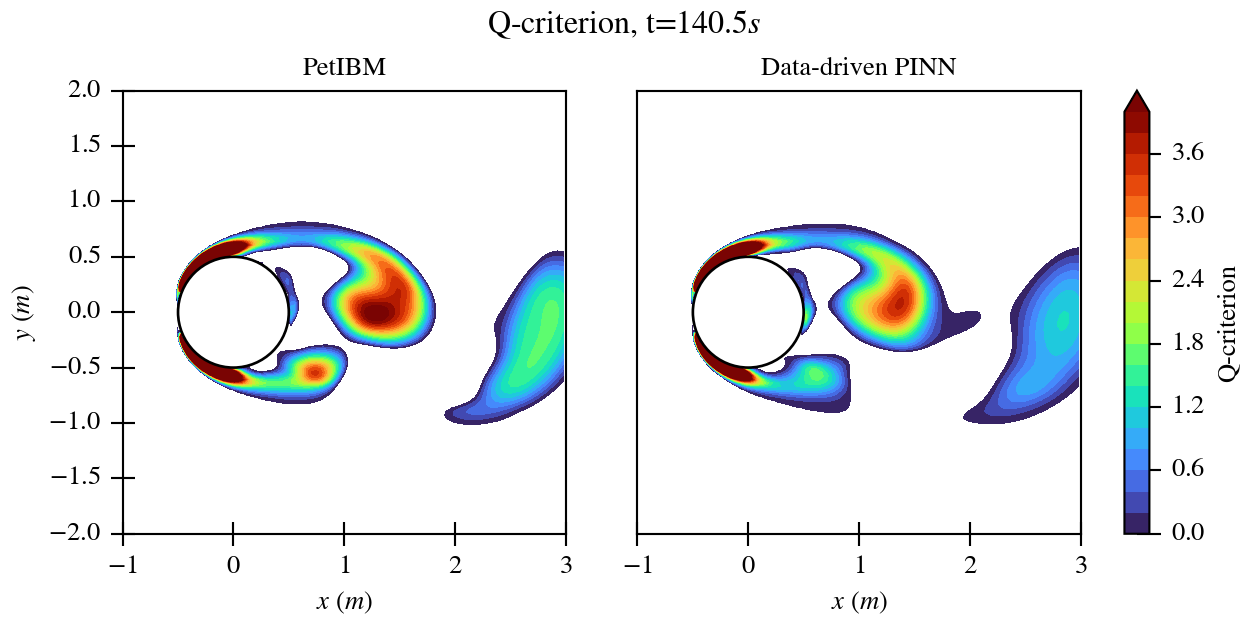
\includegraphics[width=0.95\columnwidth]{cylinder-2d-re200/qcriterion_t140.5.png}%
    \caption{%
        Q-criterion near the cylinder for 2D cylinder flow at $Re=\num{200}$ at $t=140.5$ w/ data-driven PINNs
    }
    \label{fig:cylinder-re200-pinn-qcrit-t140.5}%
\end{figure}

\begin{figure}[!hbt]
    \centering%
    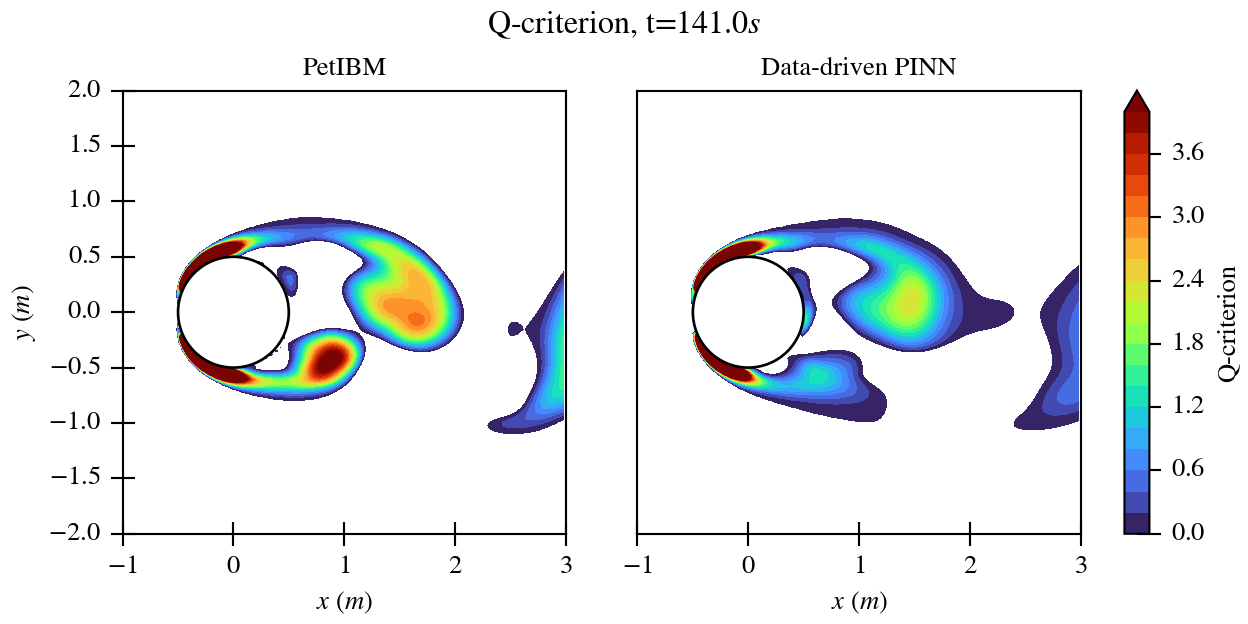
\includegraphics[width=0.95\columnwidth]{cylinder-2d-re200/qcriterion_t141.0.png}%
    \caption{%
        Q-criterion near the cylinder for 2D cylinder flow at $Re=\num{200}$ at $t=141$ w/ data-driven PINNs
    }
    \label{fig:cylinder-re200-pinn-qcrit-t141.0}%
\end{figure}

\begin{figure}[!hbt]
    \centering%
    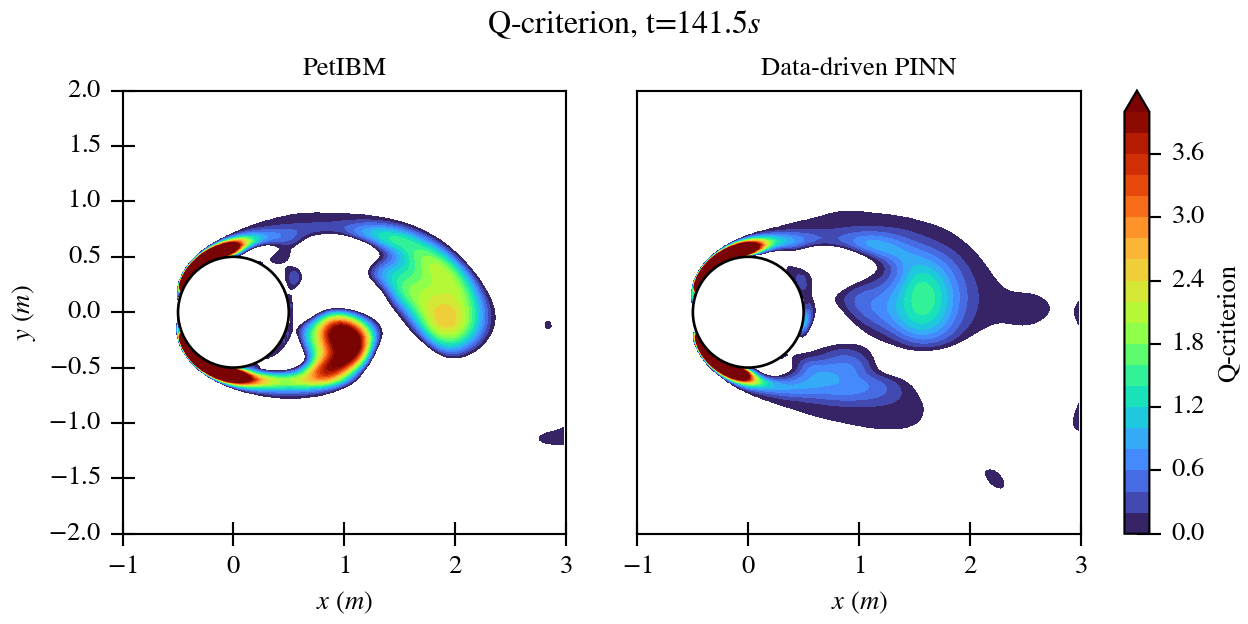
\includegraphics[width=0.95\columnwidth]{cylinder-2d-re200/qcriterion_t141.5.png}%
    \caption{%
        Q-criterion near the cylinder for 2D cylinder flow at $Re=\num{200}$ at $t=141.5$ w/ data-driven PINNs
    }
    \label{fig:cylinder-re200-pinn-qcrit-t141.5}%
\end{figure}

\begin{figure}[!hbt]
    \centering%
    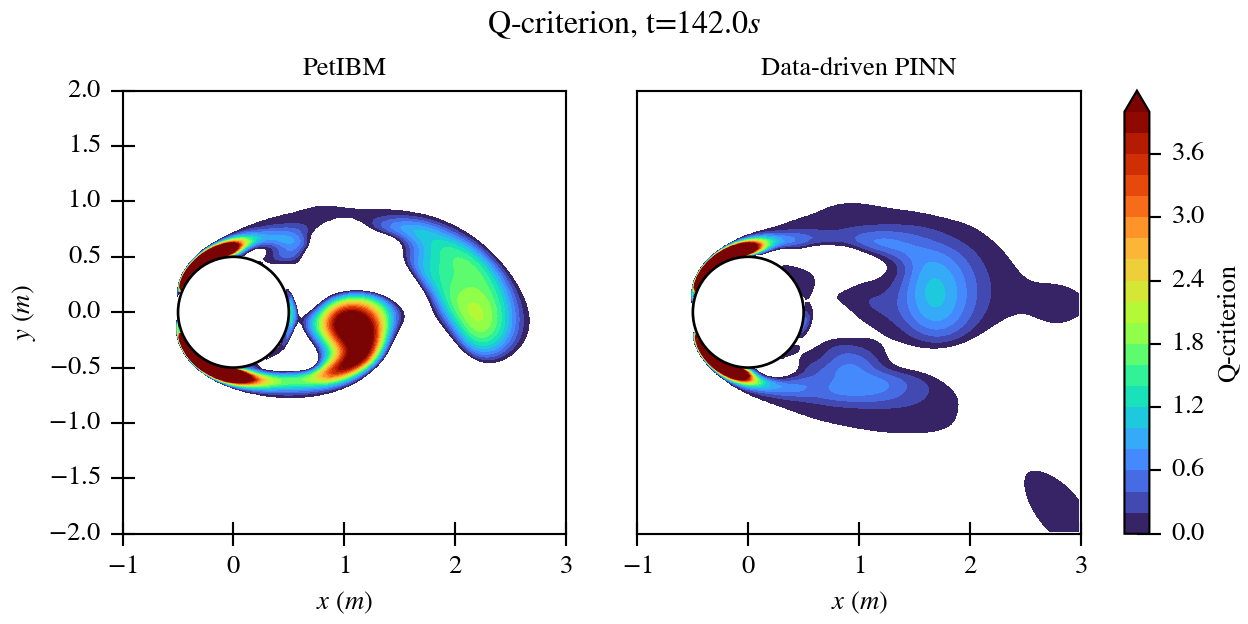
\includegraphics[width=0.95\columnwidth]{cylinder-2d-re200/qcriterion_t142.0.png}%
    \caption{%
        Q-criterion near the cylinder for 2D cylinder flow at $Re=\num{200}$ at $t=142$ w/ data-driven PINNs
    }
    \label{fig:cylinder-re200-pinn-qcrit-t142.0}%
\end{figure}

\begin{figure}[!hbt]
    \centering%
    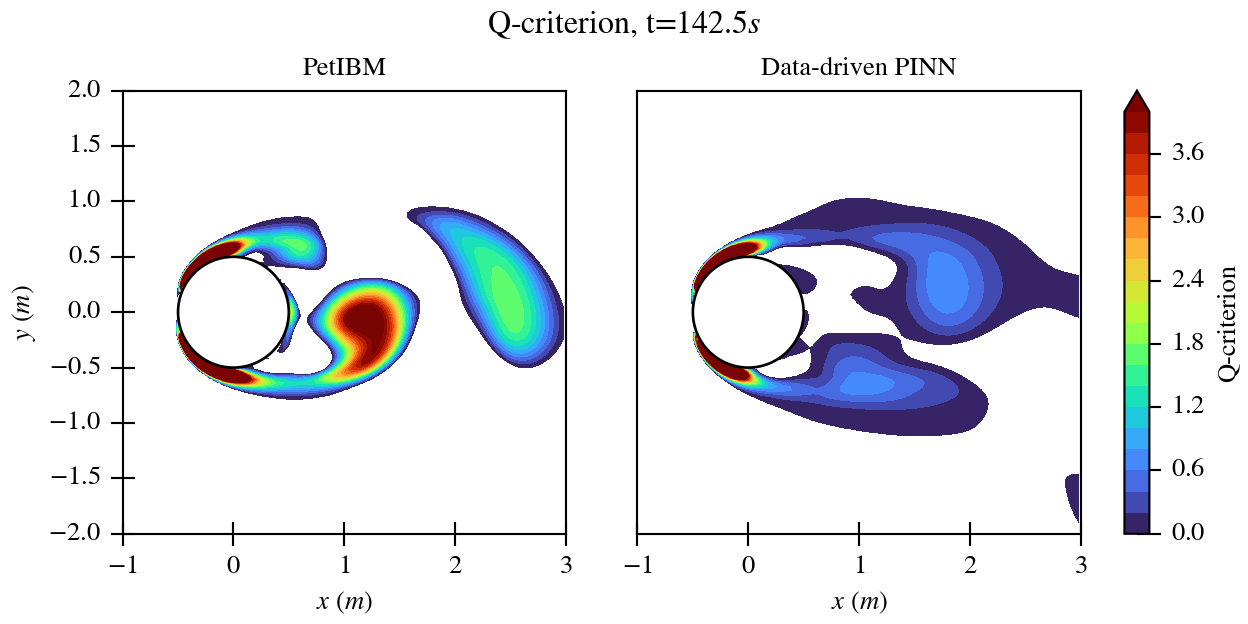
\includegraphics[width=0.95\columnwidth]{cylinder-2d-re200/qcriterion_t142.5.png}%
    \caption{%
        Q-criterion near the cylinder for 2D cylinder flow at $Re=\num{200}$ at $t=142.5$ w/ data-driven PINNs
    }
    \label{fig:cylinder-re200-pinn-qcrit-t142.5}%
\end{figure}

\begin{figure}[!hbt]
    \centering%
    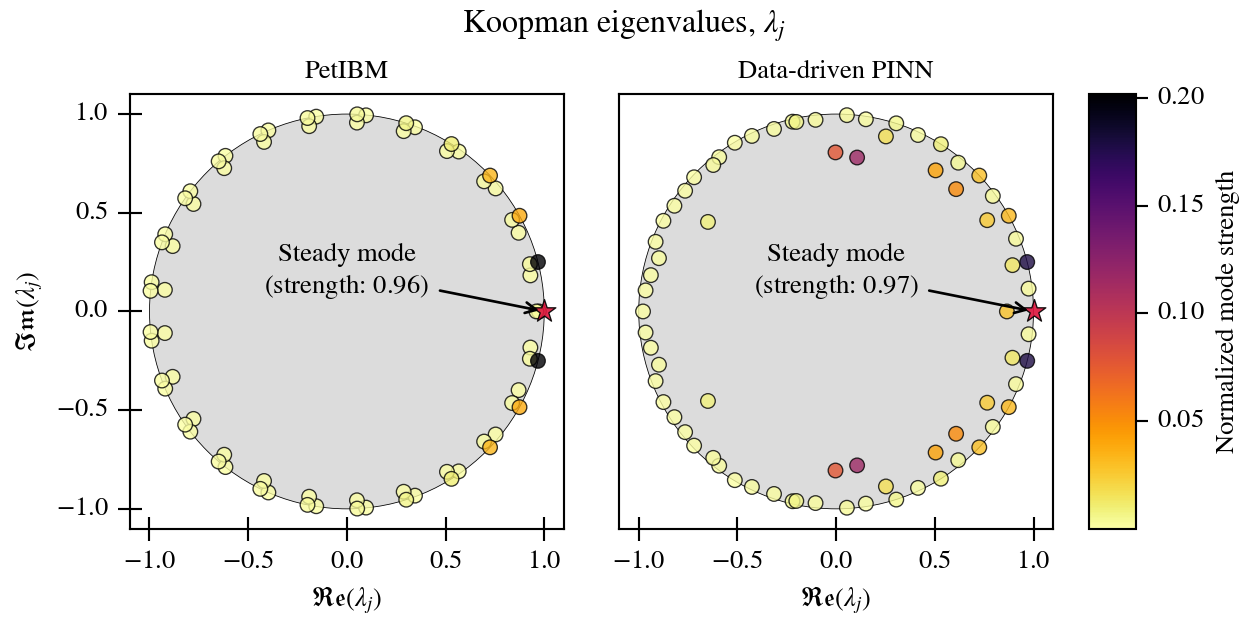
\includegraphics[width=0.95\columnwidth]{cylinder-2d-re200/koopman_eigenvalues_complex}%
    \caption{%
        Distribution of the Koopman eigenvalues on the complex plane for 2D cylinder flow at $Re=\num{200}$.
    }
    \label{fig:cylinder-re200-koopman-eig-dist}%
\end{figure}

\begin{figure}[!hbt]
    \centering%
    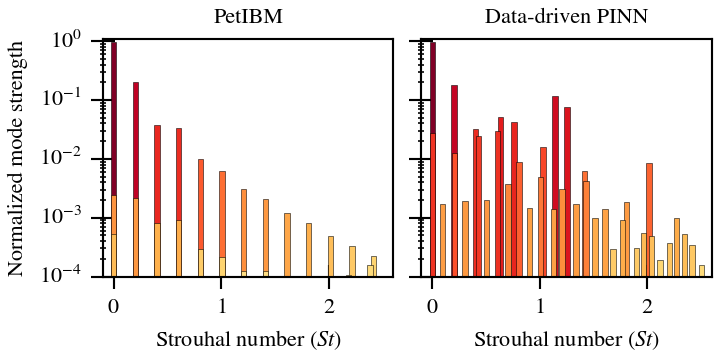
\includegraphics[width=0.95\columnwidth]{cylinder-2d-re200/koopman_mode_strength}%
    \caption{%
        Mode strengths versus mode frequencies for 2D cylinder flow at $Re=\num{200}$.
    }
    \label{fig:cylinder-re200-koopman-mode-strength}%
\end{figure}

\begin{table}[hbt!]
    \begin{threeparttable}[b]
        \begin{tabular}{ccccc}
            \toprule
            $St$ & Strength & Growth Rate & Contours \\
            \midrule
            0     & 0.96 & 1.3e-7  & Figure \ref{fig:cylinder-re200-koopman-petibm-1st}\\
            0.201 & 0.20 & -4.3e-7 & Figure \ref{fig:cylinder-re200-koopman-petibm-2nd}\\
            0.403 & 0.04 & 1.7e-6  & Figure \ref{fig:cylinder-re200-koopman-petibm-3rd}\\
            0.604 & 0.03 & 2.7e-6  & Figure \ref{fig:cylinder-re200-koopman-petibm-4th}\\
            \bottomrule
        \end{tabular}%
        \caption{%
            2D Cylinder, $Re=200$: top 4 primary dynamic modes (sorted by strengths) for PetIBM%
        }%
        \label{table:koopman-petibm}
    \end{threeparttable}
\end{table}%

\begin{table}[hbt!]
    \begin{threeparttable}[b]
        \begin{tabular}{ccccc}
            \toprule
            $St$ & Strength & Growth Rate & Contours \\
            \midrule
            0     & 0.97 & -2.2e-6  & Figure \ref{fig:cylinder-re200-koopman-pinn-primary-1st}\\
            0.201 & 0.18 & -9.4e-6  & Figure \ref{fig:cylinder-re200-koopman-pinn-primary-2nd}\\
            0.403 & 0.03 &  2.3e-5  & Figure \ref{fig:cylinder-re200-koopman-pinn-primary-3rd}\\
            0.604 & 0.03 & -8.6e-5  & Figure \ref{fig:cylinder-re200-koopman-pinn-primary-4th}\\
            \bottomrule
        \end{tabular}%
        \caption{%
            2D Cylinder, $Re=200$: top 4 primary dynamic modes (sorted by strengths) for PINN%
        }%
        \label{table:koopman-pinn-primary}
    \end{threeparttable}
\end{table}%

\begin{table}[hbt!]
    \begin{threeparttable}[b]
        \begin{tabular}{ccccc}
            \toprule
            $St$ & Strength & Growth Rate & Contours \\
            \midrule
            1.142 & 0.12 & -0.24 & Figure \ref{fig:cylinder-re200-koopman-pinn-damped-1st}\\
            1.253 & 0.08 & -0.22 & Figure \ref{fig:cylinder-re200-koopman-pinn-damped-2nd}\\
            0.633 & 0.05 & -0.14 & Figure \ref{fig:cylinder-re200-koopman-pinn-damped-3rd}\\
            0.761 & 0.04 & -0.13 & Figure \ref{fig:cylinder-re200-koopman-pinn-damped-4th}\\
            \bottomrule
        \end{tabular}%
        \caption{%
            2D Cylinder, $Re=200$: top 4 damped dynamic modes (sorted by strengths) for PINN%
        }%
        \label{table:koopman-pinn-damped}
    \end{threeparttable}
\end{table}%

\begin{figure*}[!hbt]
    \centering%
    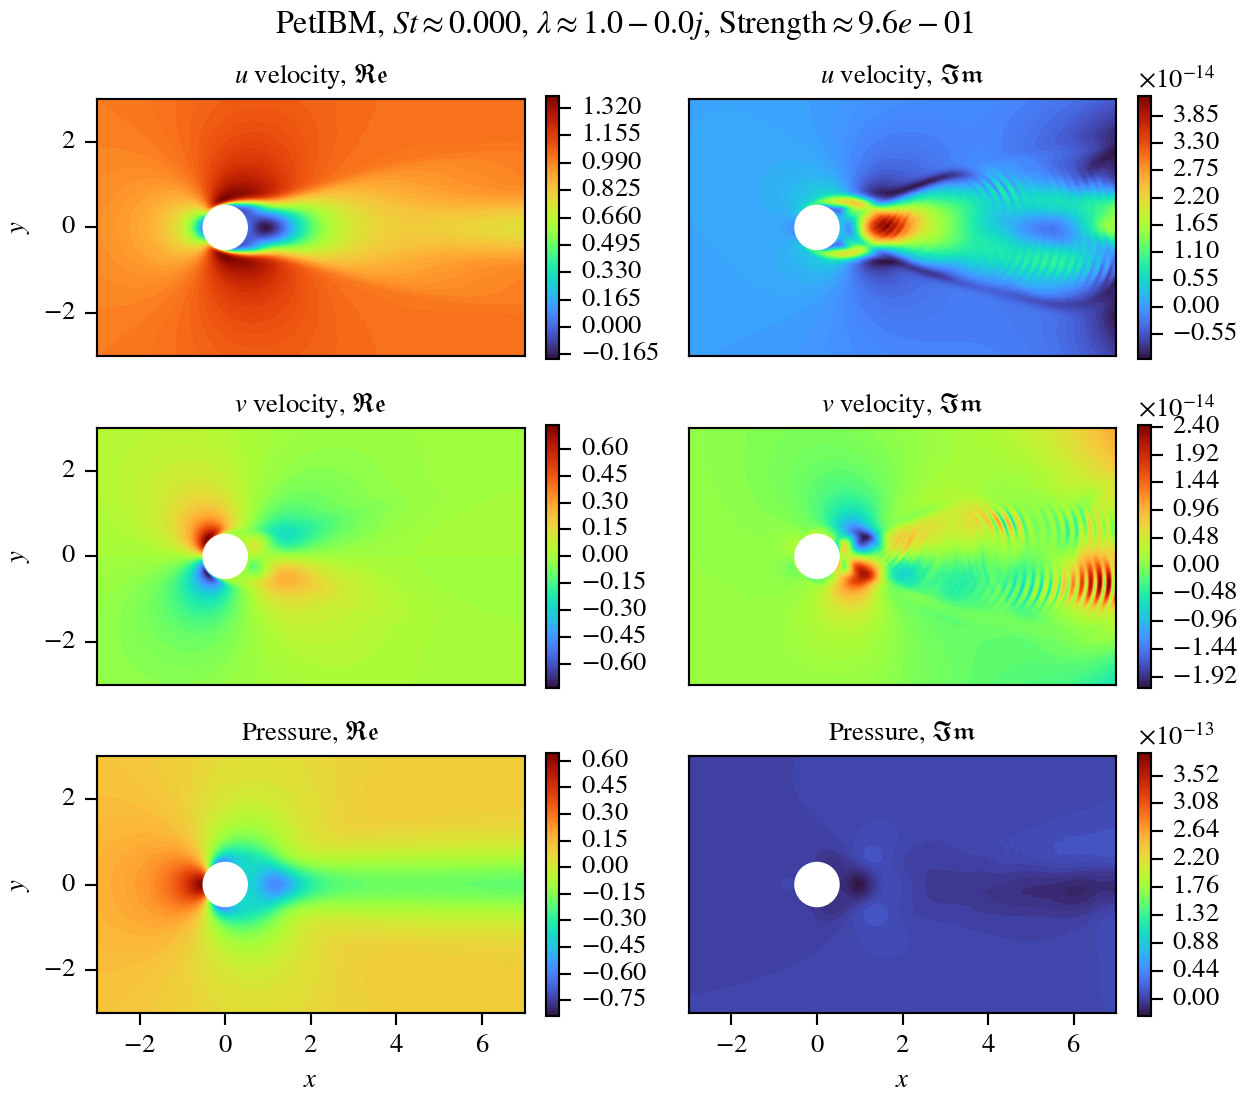
\includegraphics[width=0.8\linewidth]{cylinder-2d-re200/koopman_petibm_000_st0.000.png}%
    \caption{%
        The \num{1}st mode in PetIBM.
    }
    \label{fig:cylinder-re200-koopman-petibm-1st}%
\end{figure*}

\begin{figure*}[!hbt]
    \centering%
    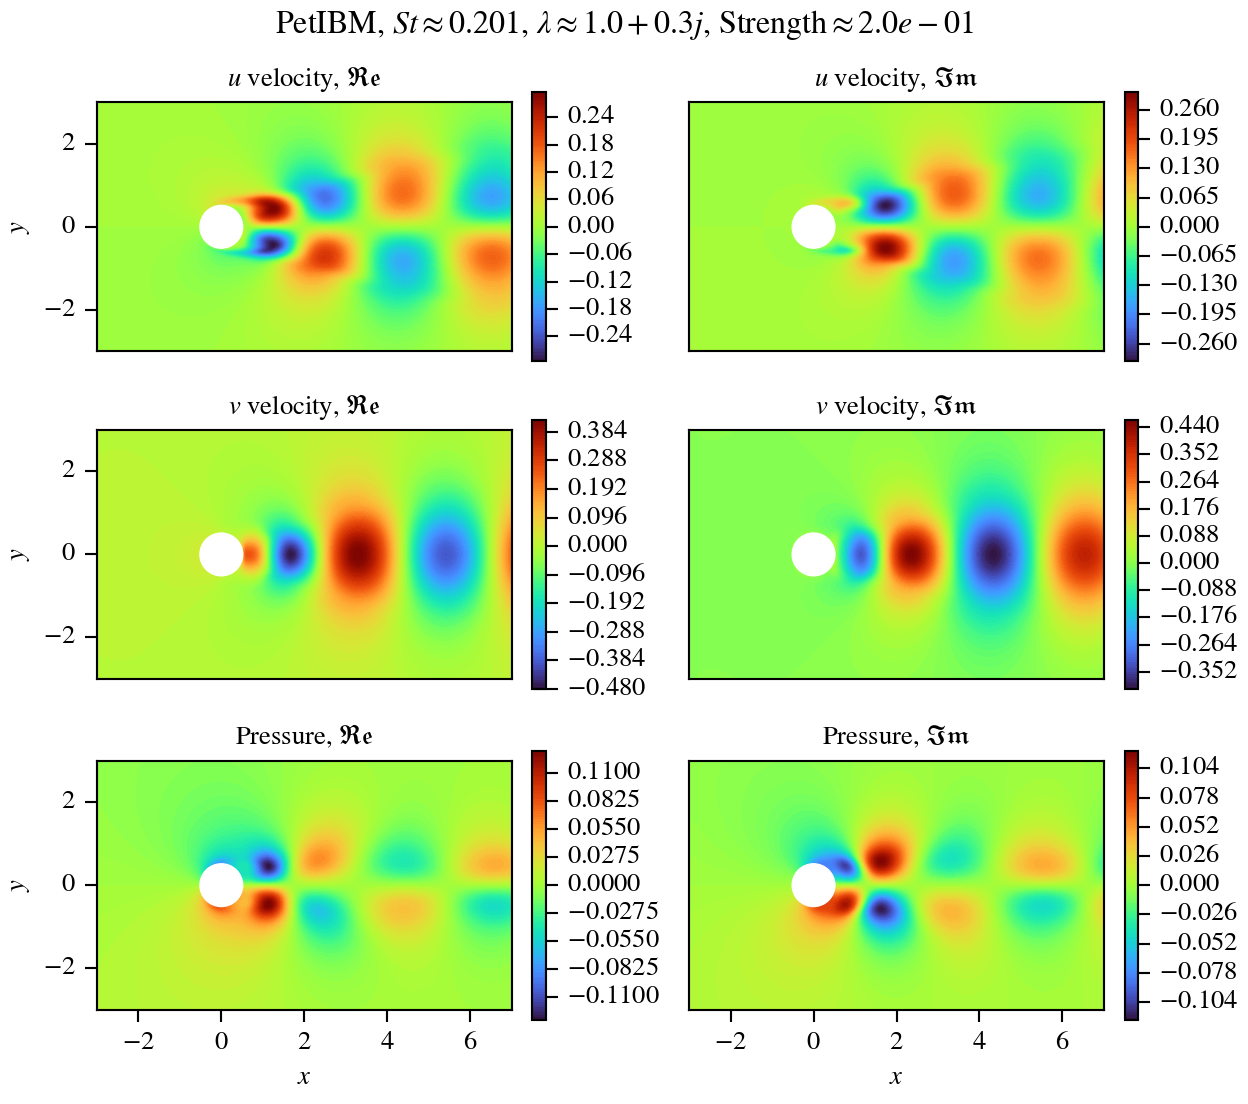
\includegraphics[width=0.8\linewidth]{cylinder-2d-re200/koopman_petibm_001_st0.201.png}%
    \caption{%
        The \num{2}nd mode in PetIBM.
    }
    \label{fig:cylinder-re200-koopman-petibm-2nd}%
\end{figure*}

\begin{figure*}[!hbt]
    \centering%
    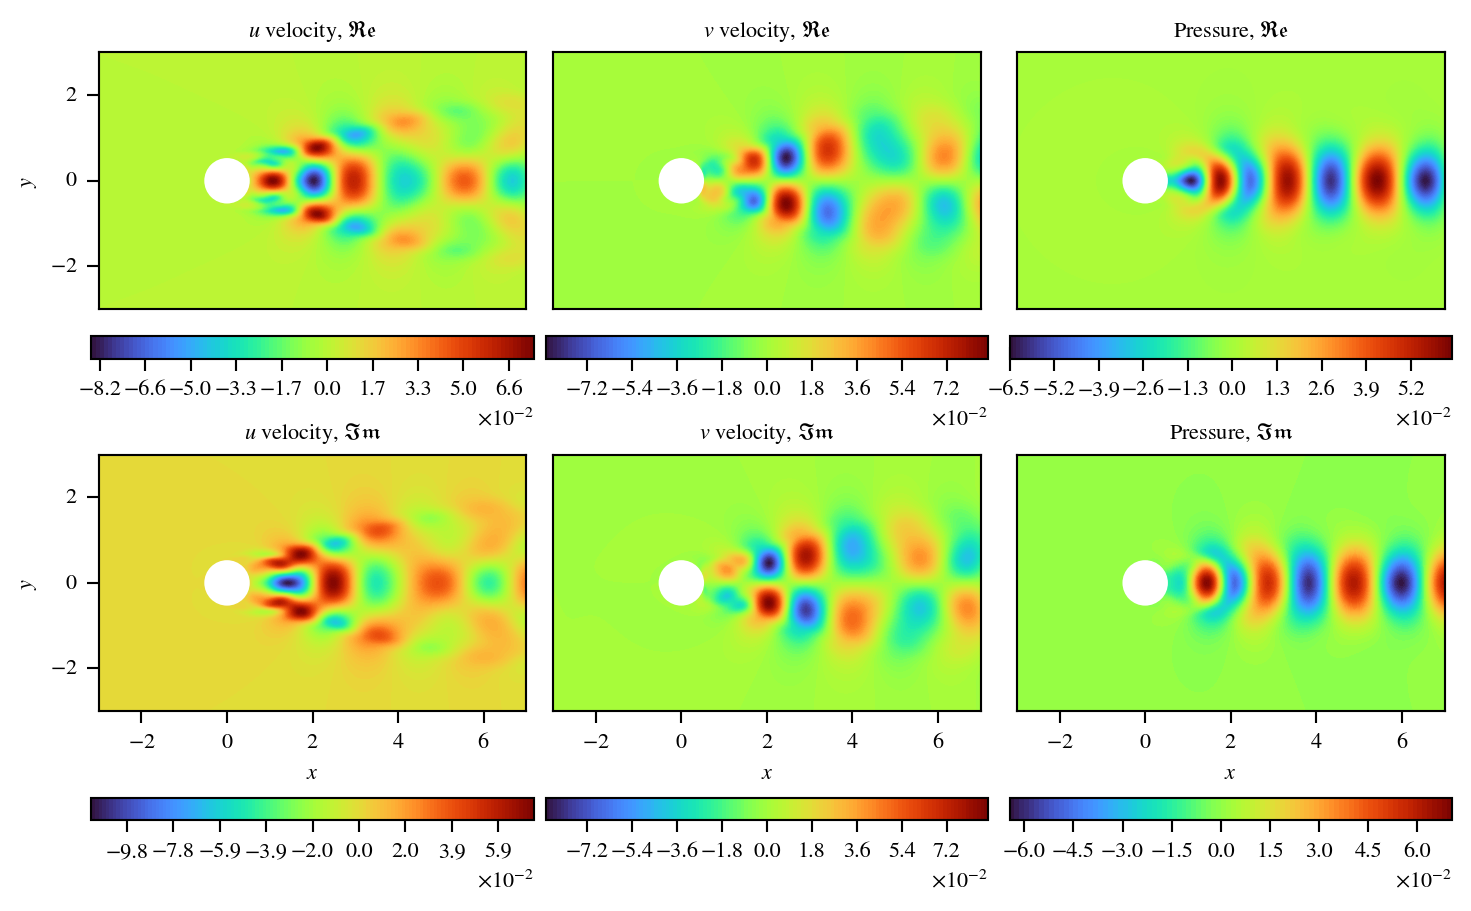
\includegraphics[width=0.8\linewidth]{cylinder-2d-re200/koopman_petibm_002_st0.403.png}%
    \caption{%
        The \num{3}rd mode in PetIBM.
    }
    \label{fig:cylinder-re200-koopman-petibm-3rd}%
\end{figure*}

\begin{figure*}[!hbt]
    \centering%
    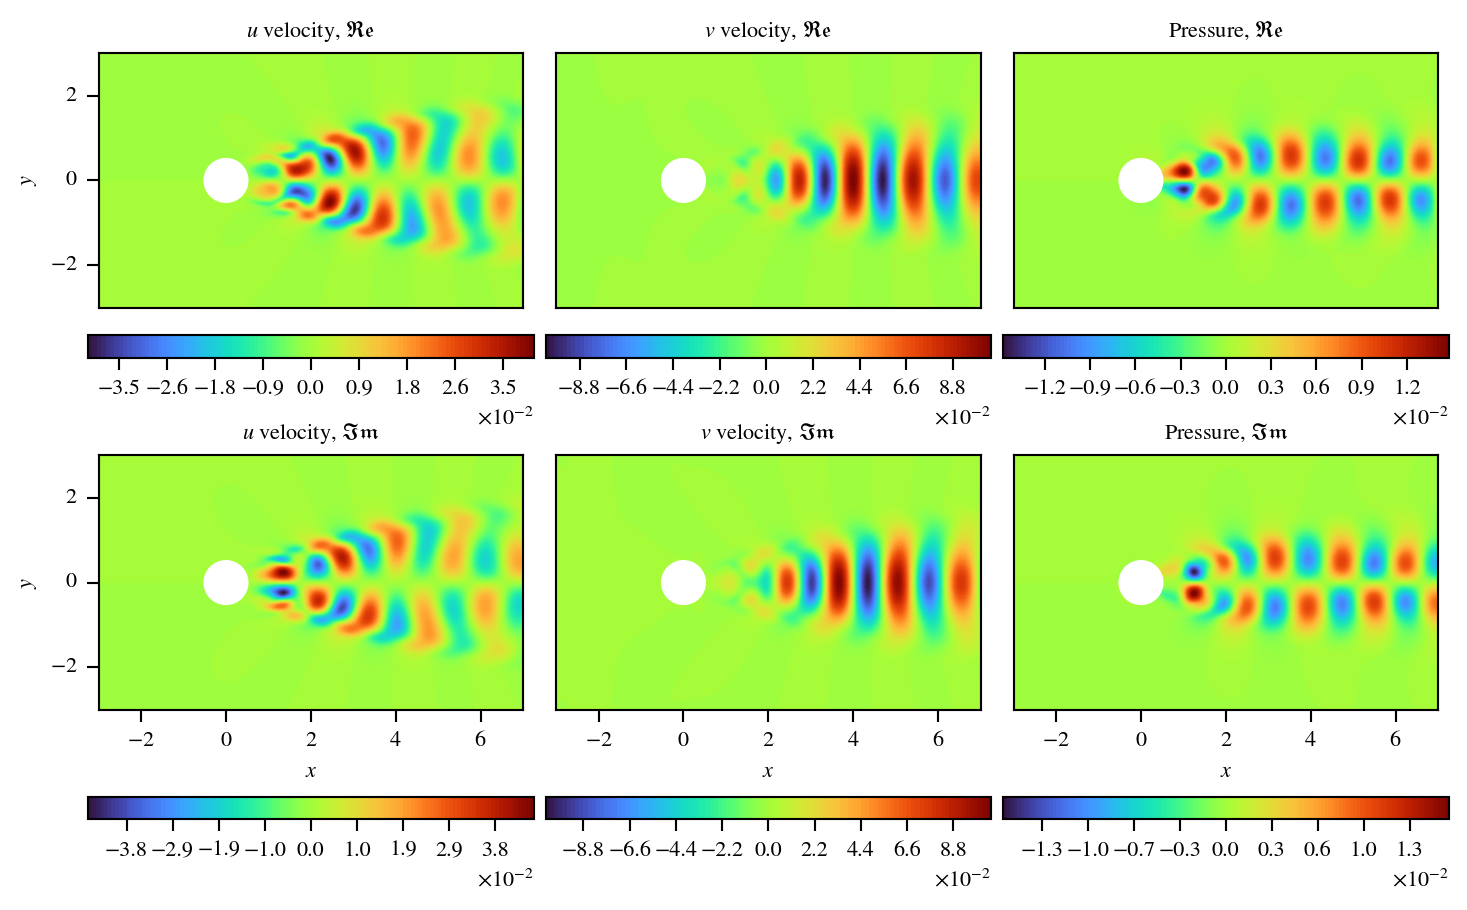
\includegraphics[width=0.8\linewidth]{cylinder-2d-re200/koopman_petibm_003_st0.604.png}%
    \caption{%
        The \num{4}th mode in PetIBM.
    }
    \label{fig:cylinder-re200-koopman-petibm-4th}%
\end{figure*}

\begin{figure*}[!hbt]
    \centering%
    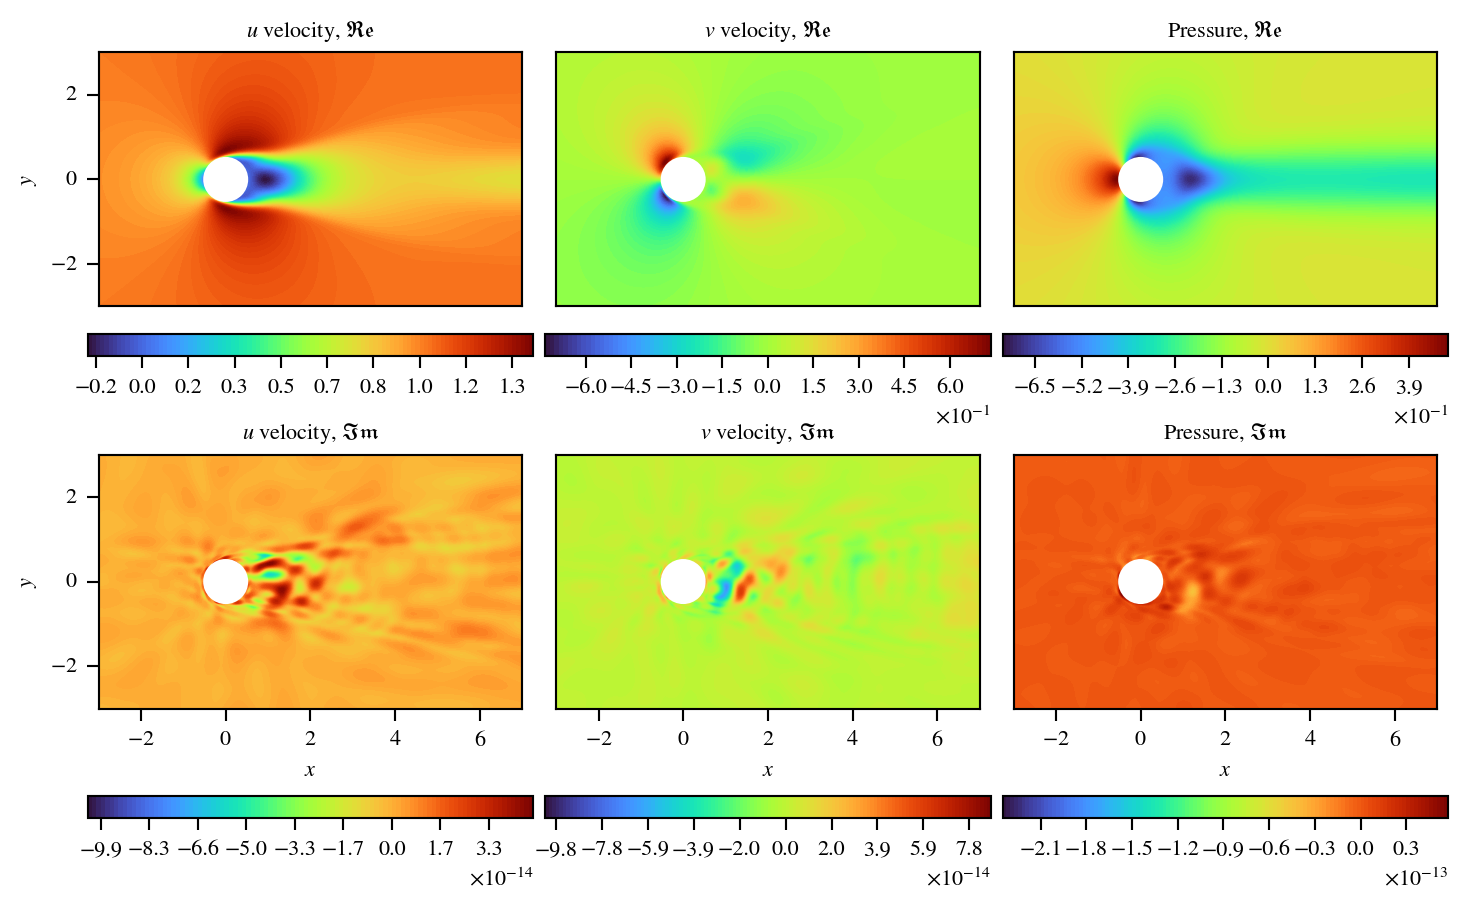
\includegraphics[width=0.8\linewidth]{cylinder-2d-re200/koopman_pinn_000_st0.000.png}%
    \caption{%
        The \num{1}st primary mode in data-driven PINN.
    }
    \label{fig:cylinder-re200-koopman-pinn-primary-1st}%
\end{figure*}

\begin{figure*}[!hbt]
    \centering%
    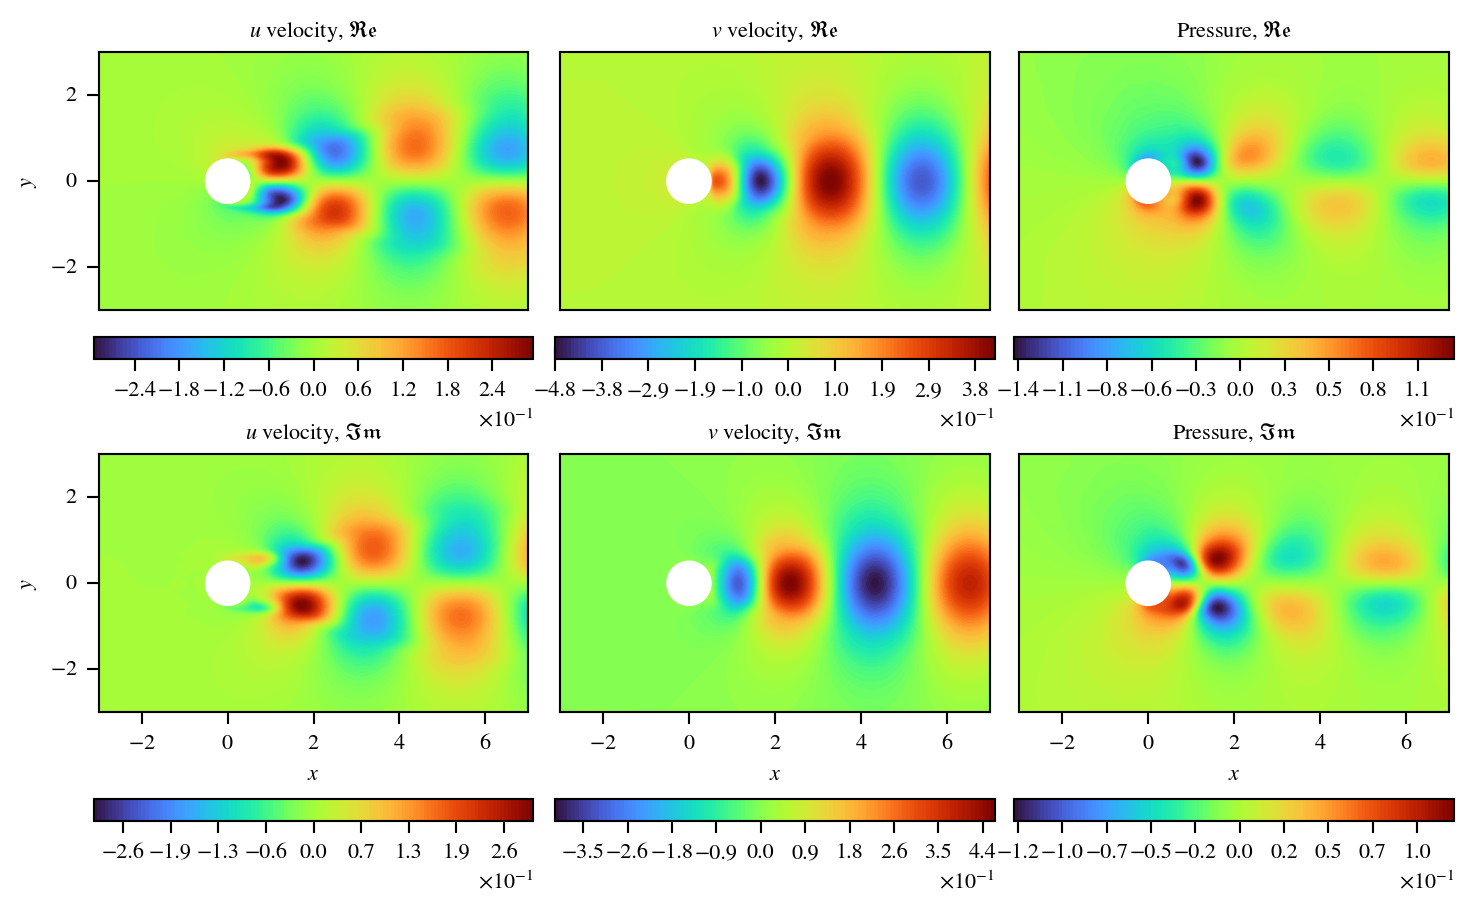
\includegraphics[width=0.8\linewidth]{cylinder-2d-re200/koopman_pinn_001_st0.201.png}%
    \caption{%
        The \num{2}nd primary mode in data-driven PINN.
    }
    \label{fig:cylinder-re200-koopman-pinn-primary-2nd}%
\end{figure*}

\begin{figure*}[!hbt]
    \centering%
    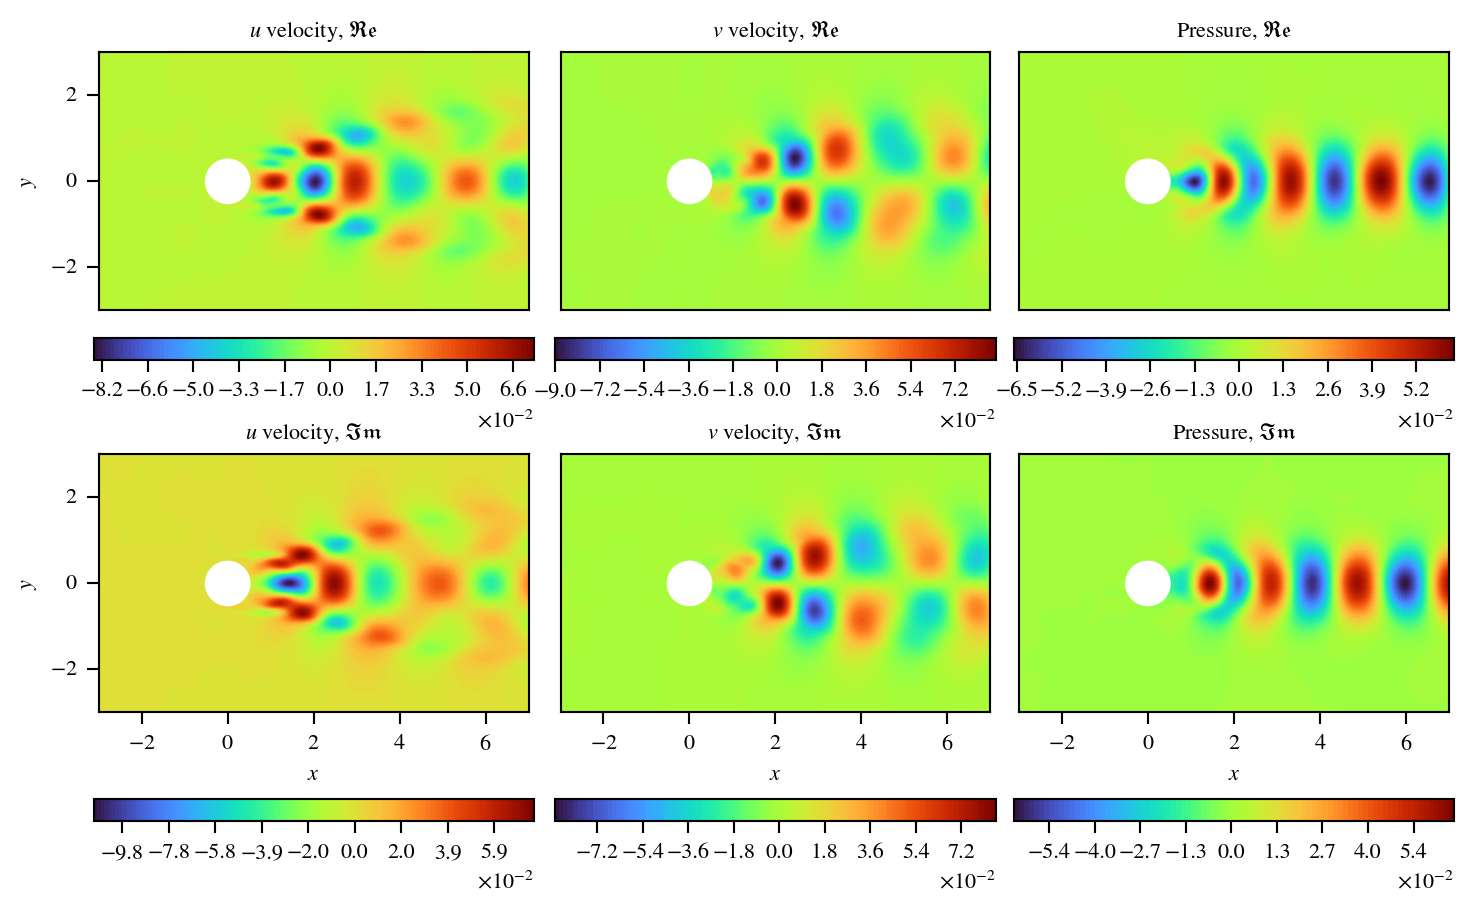
\includegraphics[width=0.8\linewidth]{cylinder-2d-re200/koopman_pinn_006_st0.403.png}%
    \caption{%
        The \num{3}rd primary mode in data-driven PINN.
    }
    \label{fig:cylinder-re200-koopman-pinn-primary-3rd}%
\end{figure*}

\begin{figure*}[!hbt]
    \centering%
    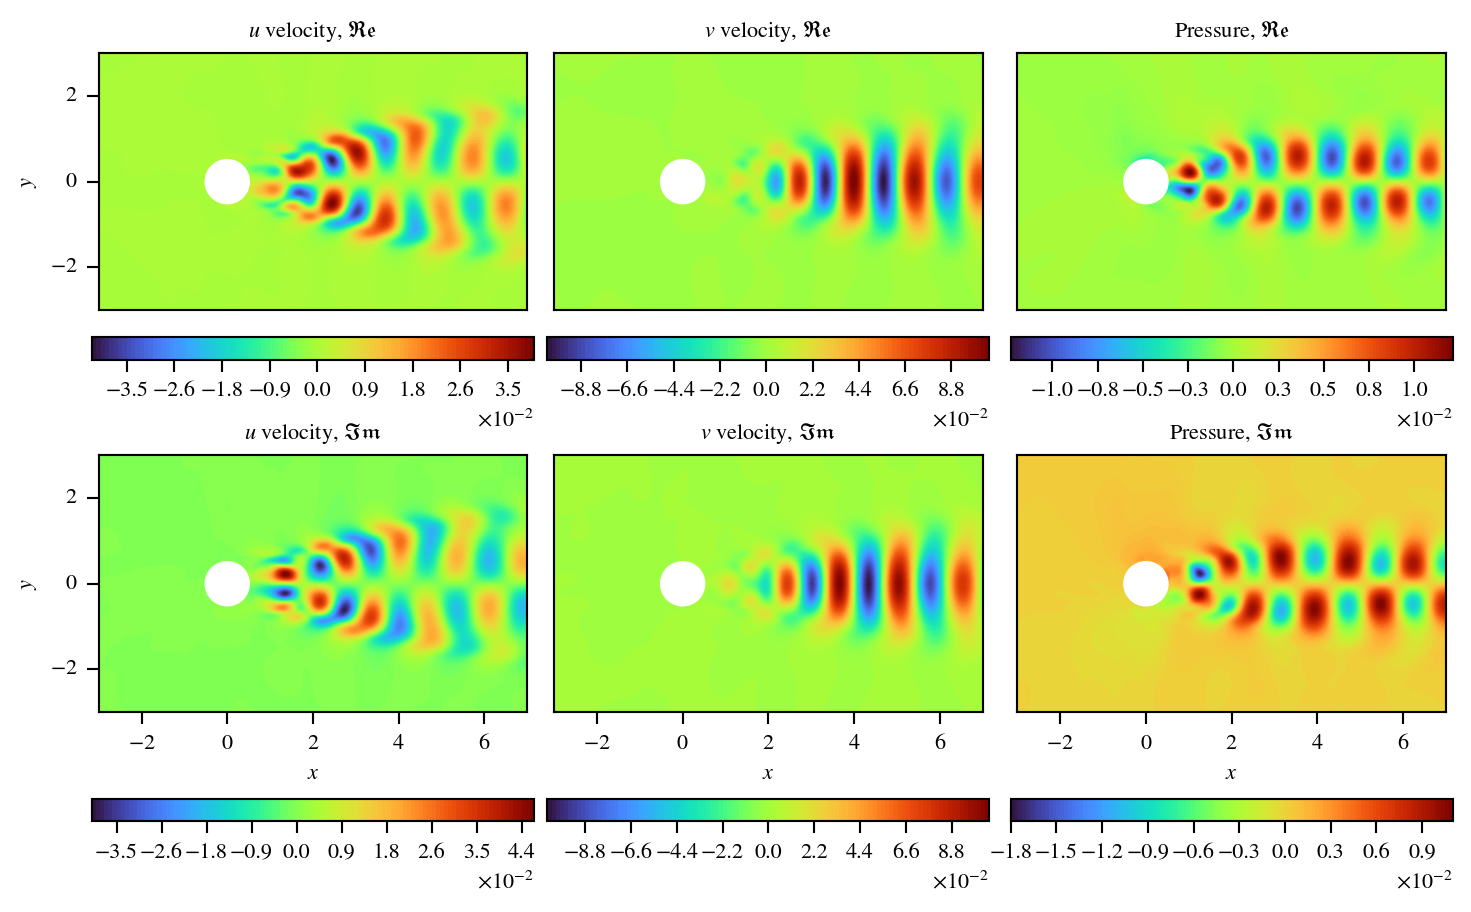
\includegraphics[width=0.8\linewidth]{cylinder-2d-re200/koopman_pinn_007_st0.604.png}%
    \caption{%
        The \num{4}th primary mode in data-driven PINN.
    }
    \label{fig:cylinder-re200-koopman-pinn-primary-4th}%
\end{figure*}

\begin{figure*}[!hbt]
    \centering%
    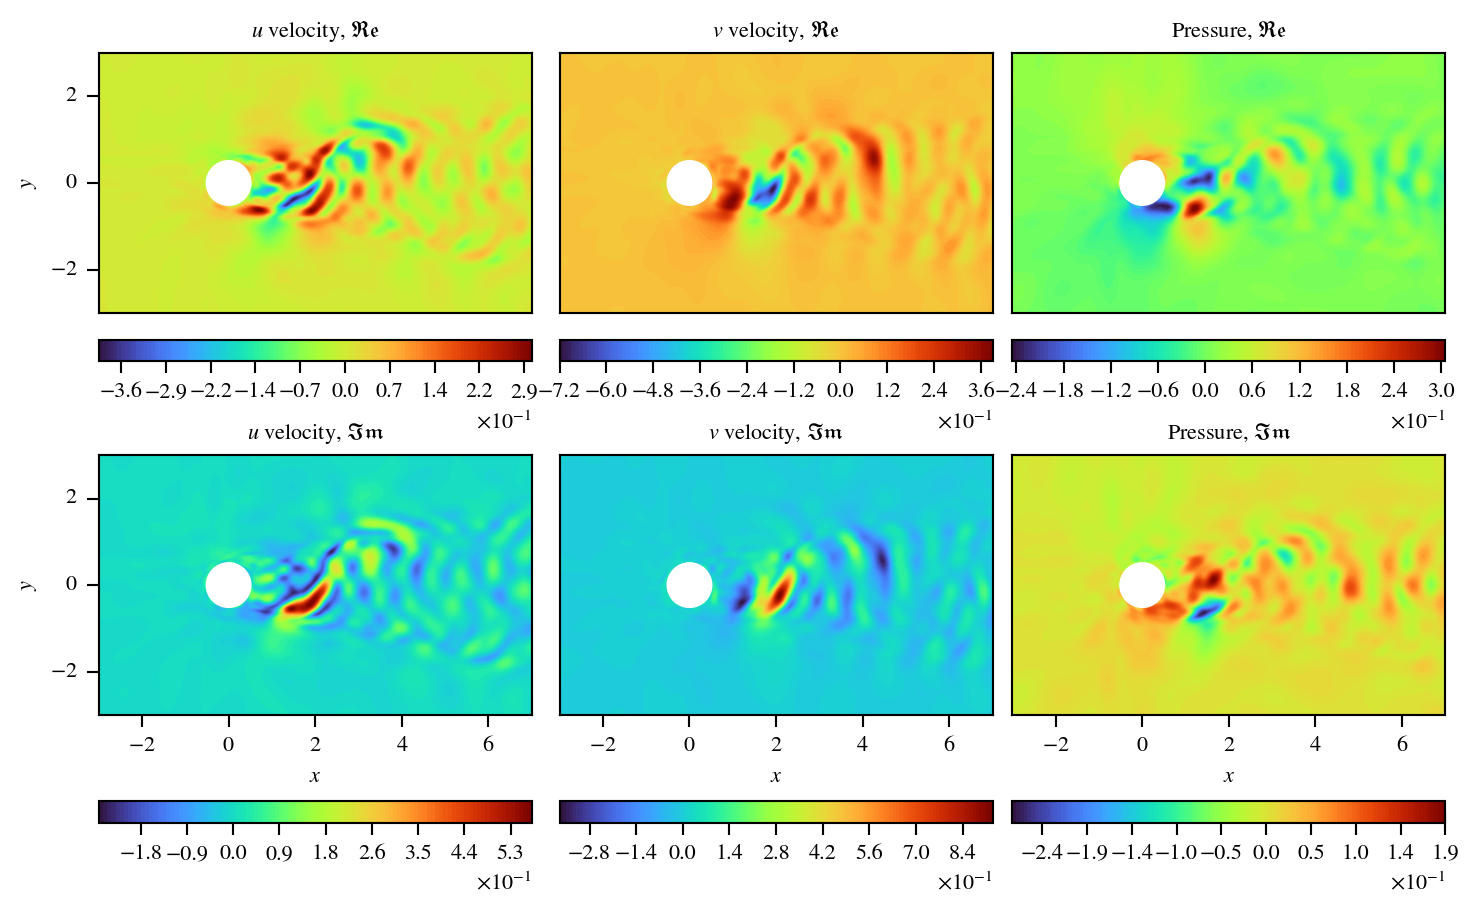
\includegraphics[width=0.8\linewidth]{cylinder-2d-re200/koopman_pinn_002_st1.142.png}%
    \caption{%
        The \num{1}st damped mode in data-driven PINN.
    }
    \label{fig:cylinder-re200-koopman-pinn-damped-1st}%
\end{figure*}

\begin{figure*}[!hbt]
    \centering%
    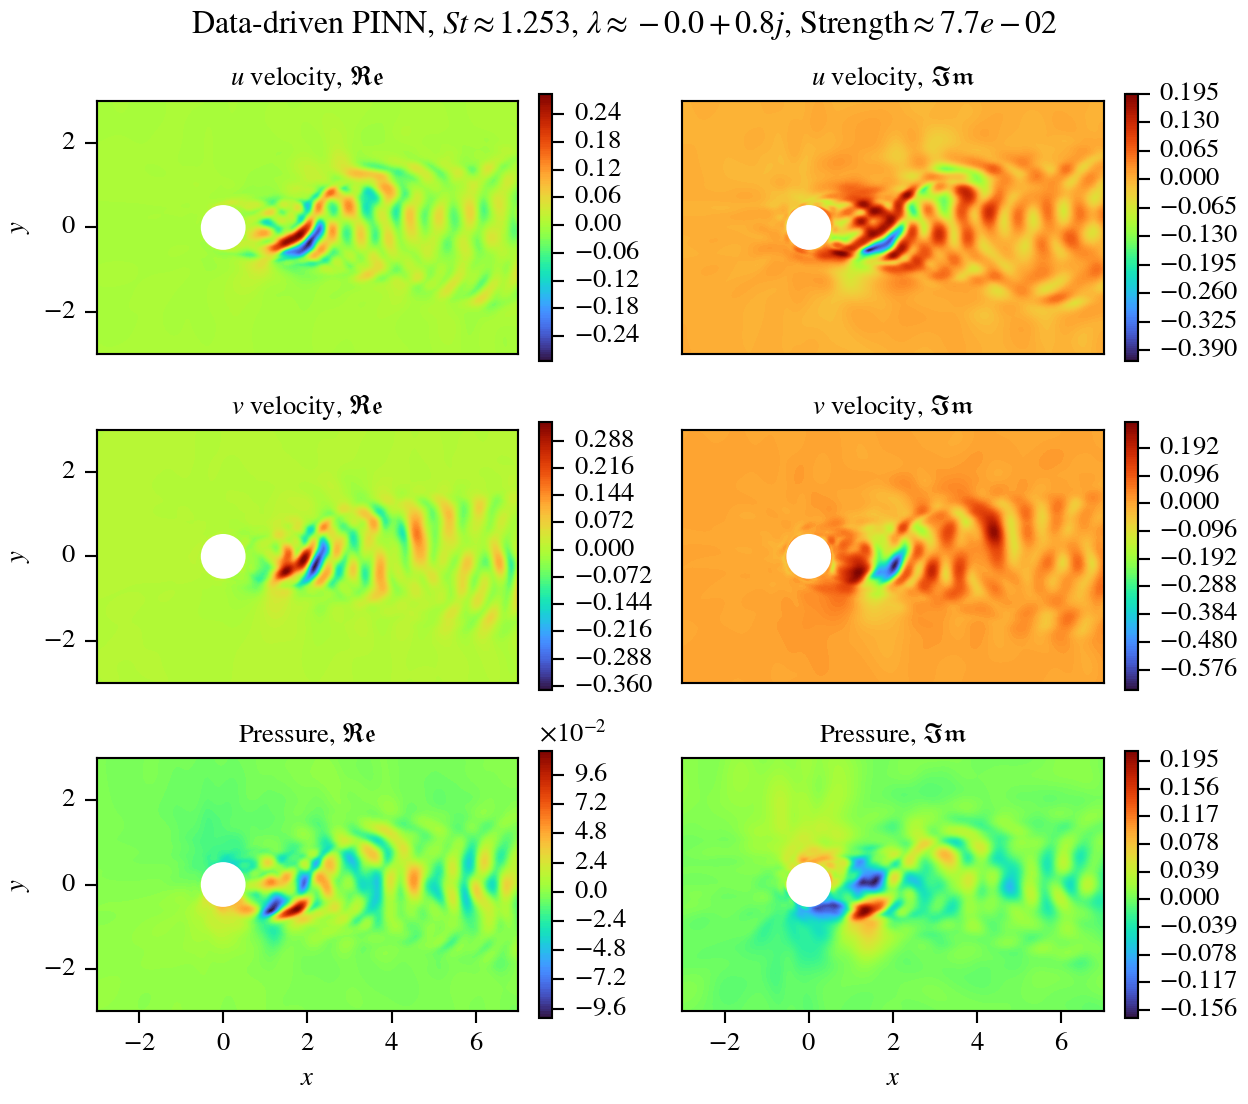
\includegraphics[width=0.8\linewidth]{cylinder-2d-re200/koopman_pinn_003_st1.253.png}%
    \caption{%
        The \num{2}nd damped mode in data-driven PINN.
    }
    \label{fig:cylinder-re200-koopman-pinn-damped-2nd}%
\end{figure*}

\begin{figure*}[!hbt]
    \centering%
    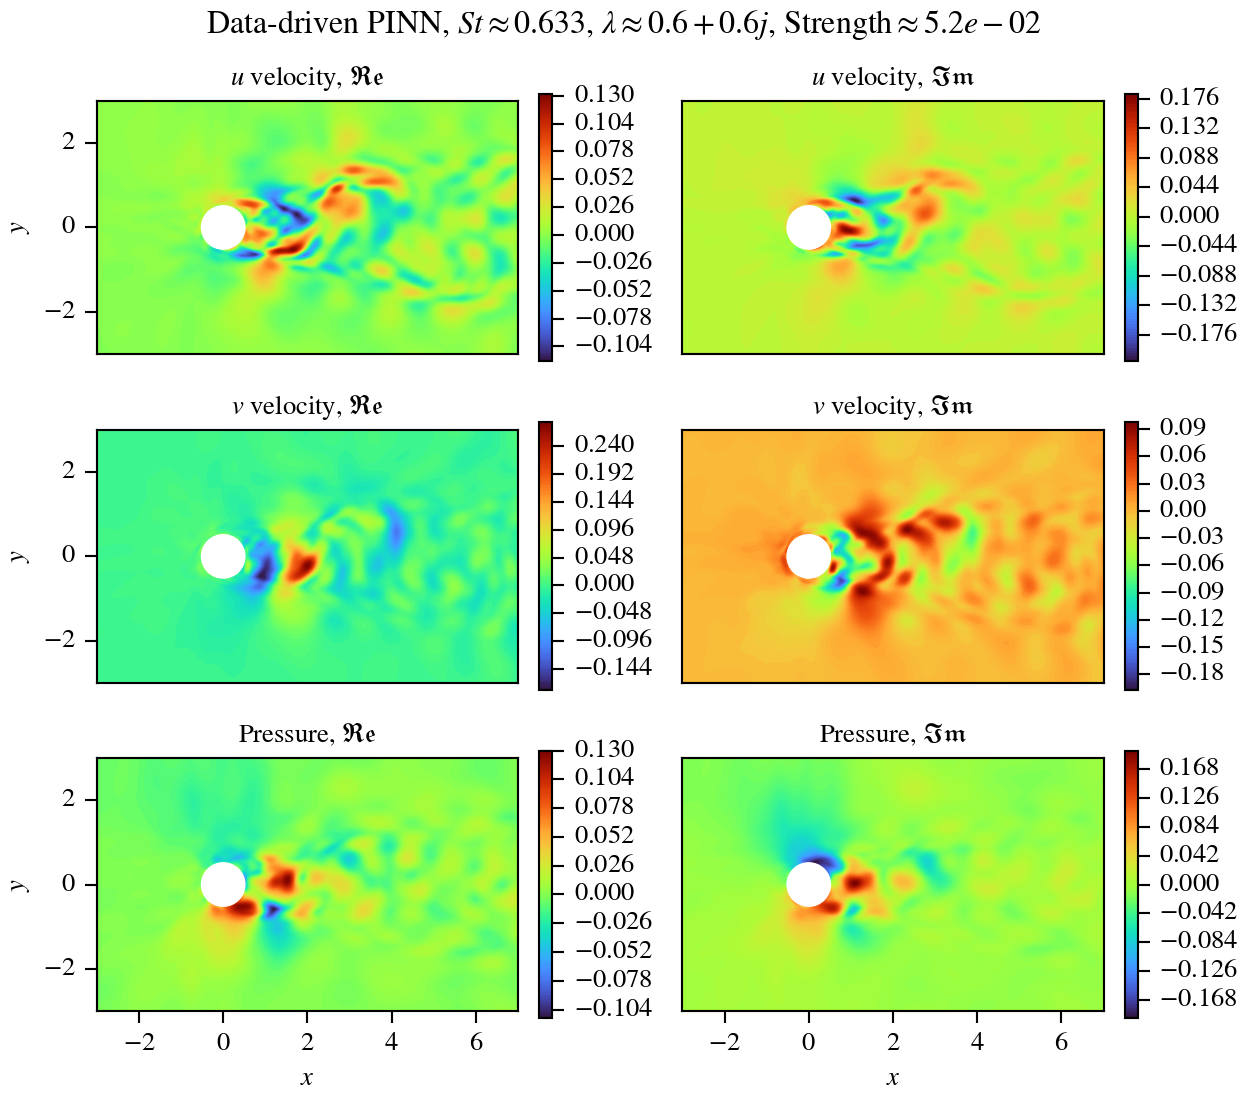
\includegraphics[width=0.8\linewidth]{cylinder-2d-re200/koopman_pinn_004_st0.633.png}%
    \caption{%
        The \num{3}rd damped mode in data-driven PINN.
    }
    \label{fig:cylinder-re200-koopman-pinn-damped-3rd}%
\end{figure*}

\begin{figure*}[!hbt]
    \centering%
    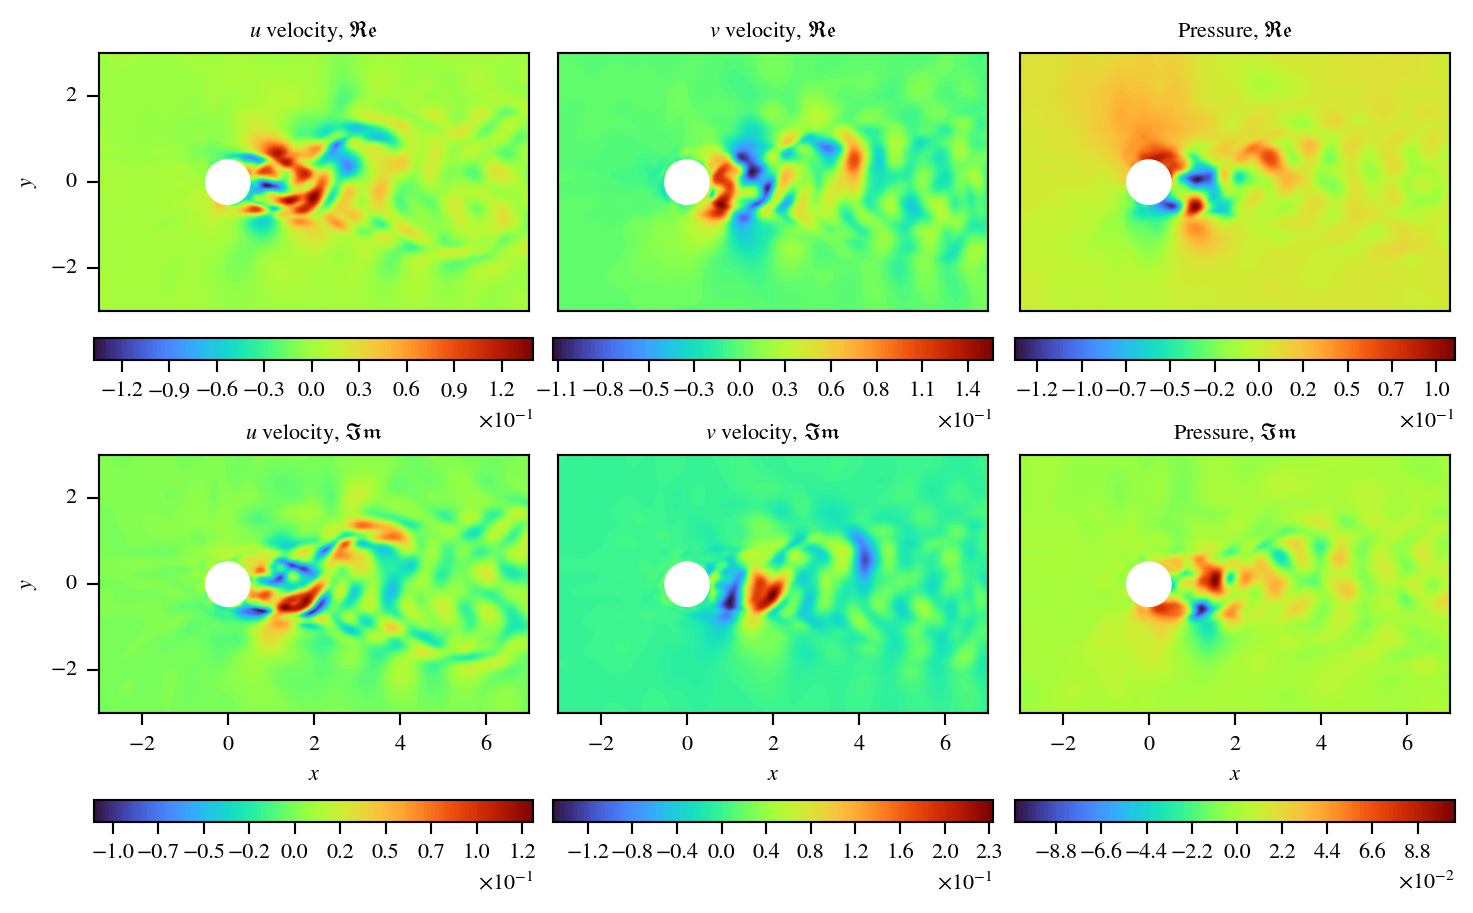
\includegraphics[width=0.8\linewidth]{cylinder-2d-re200/koopman_pinn_005_st0.761.png}%
    \caption{%
        The \num{4}th damped mode in data-driven PINN.
    }
    \label{fig:cylinder-re200-koopman-pinn-damped-4th}%
\end{figure*}

% vim:ft=tex:


    \section{Discussion}
    \lipsum[5]

    \section{Conclusion}
    \lipsum[6]

    \section*{Acknowledgement}
    \lipsum[7]

    % bibliography
    \bibliography{references}

    \appendix
    \section{Supplement}
    %! TEX root = main.tex

\begin{figure*} [h]
    \centering%
    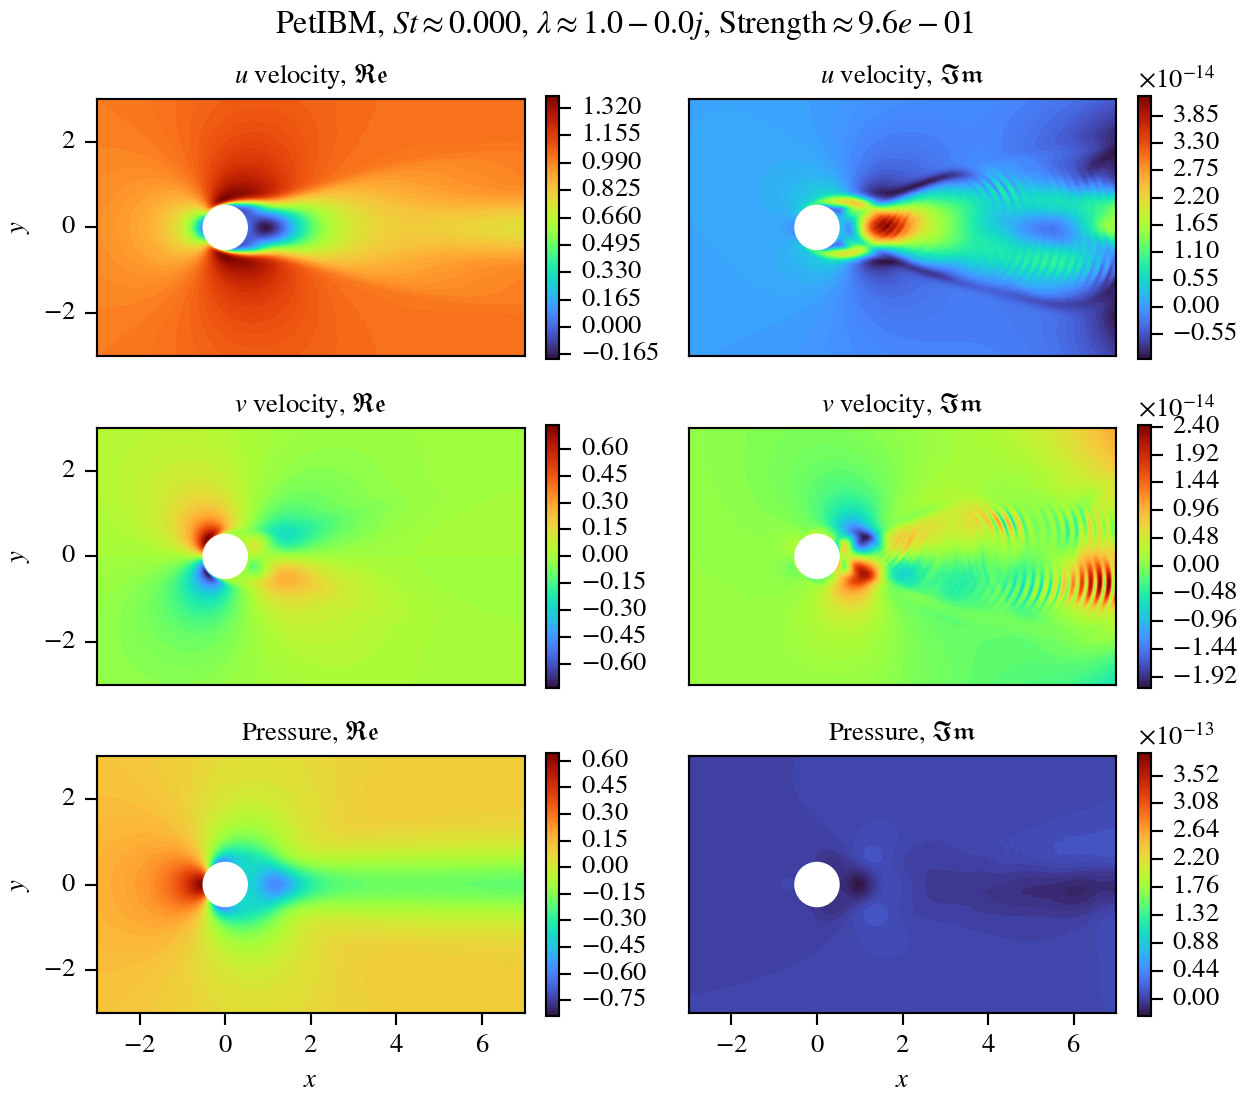
\includegraphics[width=0.95\textwidth]{cylinder-2d-re200/koopman_petibm_000_st0.000.png}%
    \caption{%
        The \num{1}st mode in PetIBM.
    }
    \label{fig:cylinder-re200-koopman-petibm-1st}%
\end{figure*}

\begin{figure*} 
    \centering%
    \includegraphics[width=0.95\textwidth]{cylinder-2d-re200/koopman_petibm_001_st0.201.png}%
    \caption{%
        The \num{2}nd mode in PetIBM.
    }
    \label{fig:cylinder-re200-koopman-petibm-2nd}%
\end{figure*}

\begin{figure*} 
    \centering%
    \includegraphics[width=0.95\textwidth]{cylinder-2d-re200/koopman_petibm_002_st0.403.png}%
    \caption{%
        The \num{3}rd mode in PetIBM.
    }
    \label{fig:cylinder-re200-koopman-petibm-3rd}%
\end{figure*}

\begin{figure*} 
    \centering%
    \includegraphics[width=0.95\textwidth]{cylinder-2d-re200/koopman_petibm_003_st0.604.png}%
    \caption{%
        The \num{4}th mode in PetIBM.
    }
    \label{fig:cylinder-re200-koopman-petibm-4th}%
\end{figure*}

\begin{figure*} 
    \centering%
    \includegraphics[width=0.95\textwidth]{cylinder-2d-re200/koopman_pinn_000_st0.000.png}%
    \caption{%
        The \num{1}st primary mode in data-driven PINN.
    }
    \label{fig:cylinder-re200-koopman-pinn-primary-1st}%
\end{figure*}

\begin{figure*} 
    \centering%
    \includegraphics[width=0.95\textwidth]{cylinder-2d-re200/koopman_pinn_001_st0.201.png}%
    \caption{%
        The \num{2}nd primary mode in data-driven PINN.
    }
    \label{fig:cylinder-re200-koopman-pinn-primary-2nd}%
\end{figure*}

\begin{figure*} 
    \centering%
    \includegraphics[width=0.95\textwidth]{cylinder-2d-re200/koopman_pinn_006_st0.403.png}%
    \caption{%
        The \num{3}rd primary mode in data-driven PINN.
    }
    \label{fig:cylinder-re200-koopman-pinn-primary-3rd}%
\end{figure*}

\begin{figure*} 
    \centering%
    \includegraphics[width=0.95\textwidth]{cylinder-2d-re200/koopman_pinn_007_st0.604.png}%
    \caption{%
        The \num{4}th primary mode in data-driven PINN.
    }
    \label{fig:cylinder-re200-koopman-pinn-primary-4th}%
\end{figure*}

\begin{figure*} 
    \centering%
    \includegraphics[width=0.95\textwidth]{cylinder-2d-re200/koopman_pinn_002_st1.142.png}%
    \caption{%
        The \num{1}st damped mode in data-driven PINN.
    }
    \label{fig:cylinder-re200-koopman-pinn-damped-1st}%
\end{figure*}

\begin{figure*} 
    \centering%
    \includegraphics[width=0.95\textwidth]{cylinder-2d-re200/koopman_pinn_003_st1.253.png}%
    \caption{%
        The \num{2}nd damped mode in data-driven PINN.
    }
    \label{fig:cylinder-re200-koopman-pinn-damped-2nd}%
\end{figure*}

\begin{figure*} 
    \centering%
    \includegraphics[width=0.95\textwidth]{cylinder-2d-re200/koopman_pinn_004_st0.633.png}%
    \caption{%
        The \num{3}rd damped mode in data-driven PINN.
    }
    \label{fig:cylinder-re200-koopman-pinn-damped-3rd}%
\end{figure*}

\begin{figure*} 
    \centering%
    \includegraphics[width=0.95\textwidth]{cylinder-2d-re200/koopman_pinn_005_st0.761.png}%
    \caption{%
        The \num{4}th damped mode in data-driven PINN.
    }
    \label{fig:cylinder-re200-koopman-pinn-damped-4th}%
\end{figure*}

% vim:ft=tex:

\end{document}
% vim:ft=tex:
